\section{Numerische L"osung\label{section:lorenz2:numeric-solution}}
\rhead{Numerische L"osung}
Mit den \cref{equation:lorenz2:dota,equation:lorenz2:dotb} aus 
\cref{section:lorenz2:ho-model} haben wir Gleichungen gefunden, die wir 
mit einem Computer-Algebra Programm, wie beispielsweise \texttt{maxima}, 
generiert und dann mit einem ODE-Solver, zum Beispiel \texttt{lsode} in 
\texttt{octave}, gel"ost werden k"onnen.

Das L"osen dieser Gleichungssysteme hat sich als "ausserst Zeitintensiv 
herausgestellt. Selbst nach einigen Optimierungen dauerte es "uber eine Woche 
um einzelne Systeme zu l"osen, was \cref{figure:lorenz2:timings} zeigt. F"ur 
die Systeme $k = \{2,3,\dots,22\}$ wurden die Berechnungen f"ur ein mit Grad $k 
= 2$ chaotischem Lorenzsystem durchgef"uhrt 
(\cref{figure:lorenz2:systemdeg2,figure:lorenz2:systemdeg3,figure:lorenz2:systemdeg4,figure:lorenz2:systemdeg5,figure:lorenz2:systemdeg6,figure:lorenz2:systemdeg7,figure:lorenz2:systemdeg8,figure:lorenz2:systemdeg9,figure:lorenz2:systemdeg10,figure:lorenz2:systemdeg11,figure:lorenz2:systemdeg12,figure:lorenz2:systemdeg13,figure:lorenz2:systemdeg14,figure:lorenz2:systemdeg15,figure:lorenz2:systemdeg16,figure:lorenz2:systemdeg17,figure:lorenz2:systemdeg18,figure:lorenz2:systemdeg19,figure:lorenz2:systemdeg20,figure:lorenz2:systemdeg21-40,figure:lorenz2:systemdeg22-40}).

Auff"allig ist, das ab $k = 4$ das chaotische Verhalten verschwindet. Das 
k"onnte einerseits daran liegen, dass unsere Reduktion des Ursprungssystems 
dazu gef"uhrt hat. Andererseits muss auch gesagt werden, dass wir keine 
Variation unserer Parameter und Anfangsbedingungen durchgef"uhrt haben, indem 
wir alle mit gr"osserem Grad $k$ dazugekommenen Anfangsbedingungen gleich 0 
gesetzt haben.

\begin{figure}
	\centering
	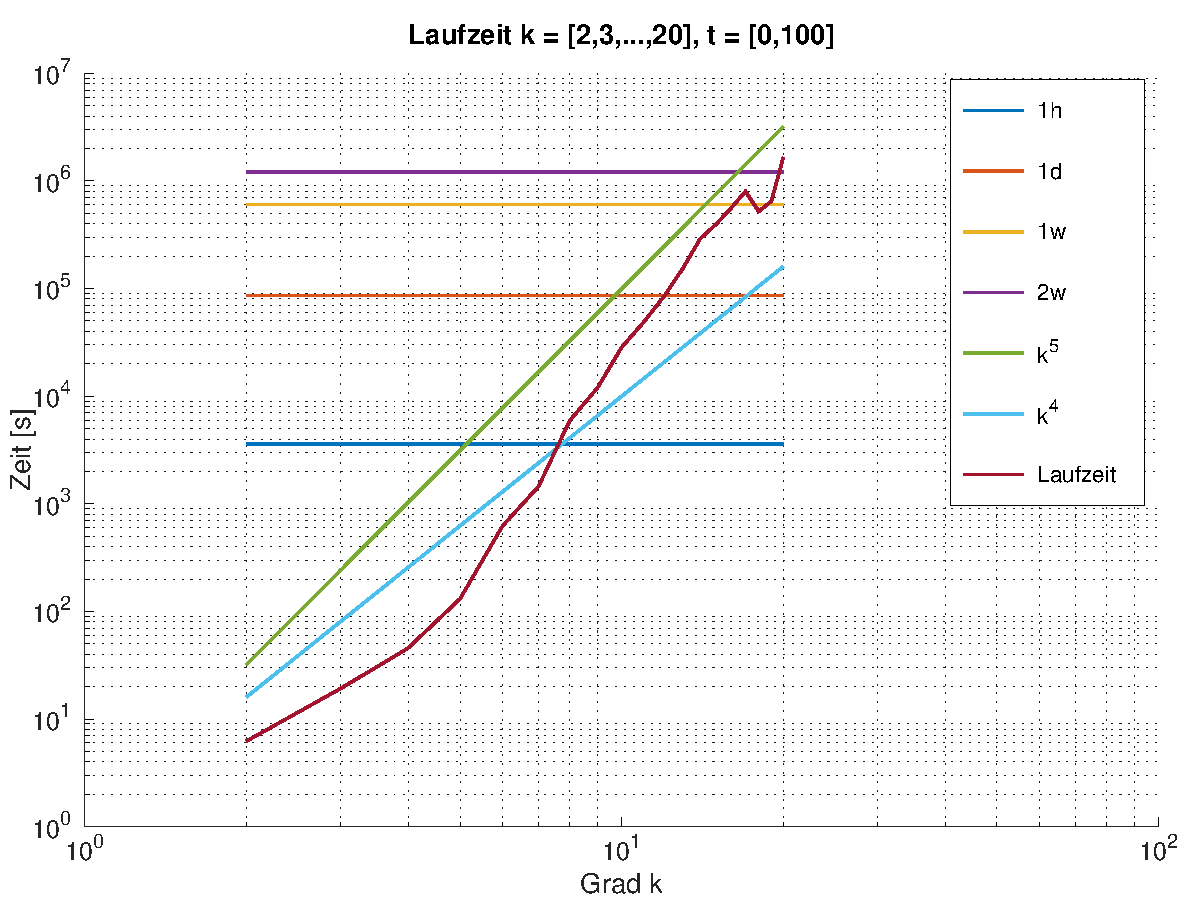
\includegraphics[width=0.49\linewidth]{lorenz2/03-images/timing_100}
	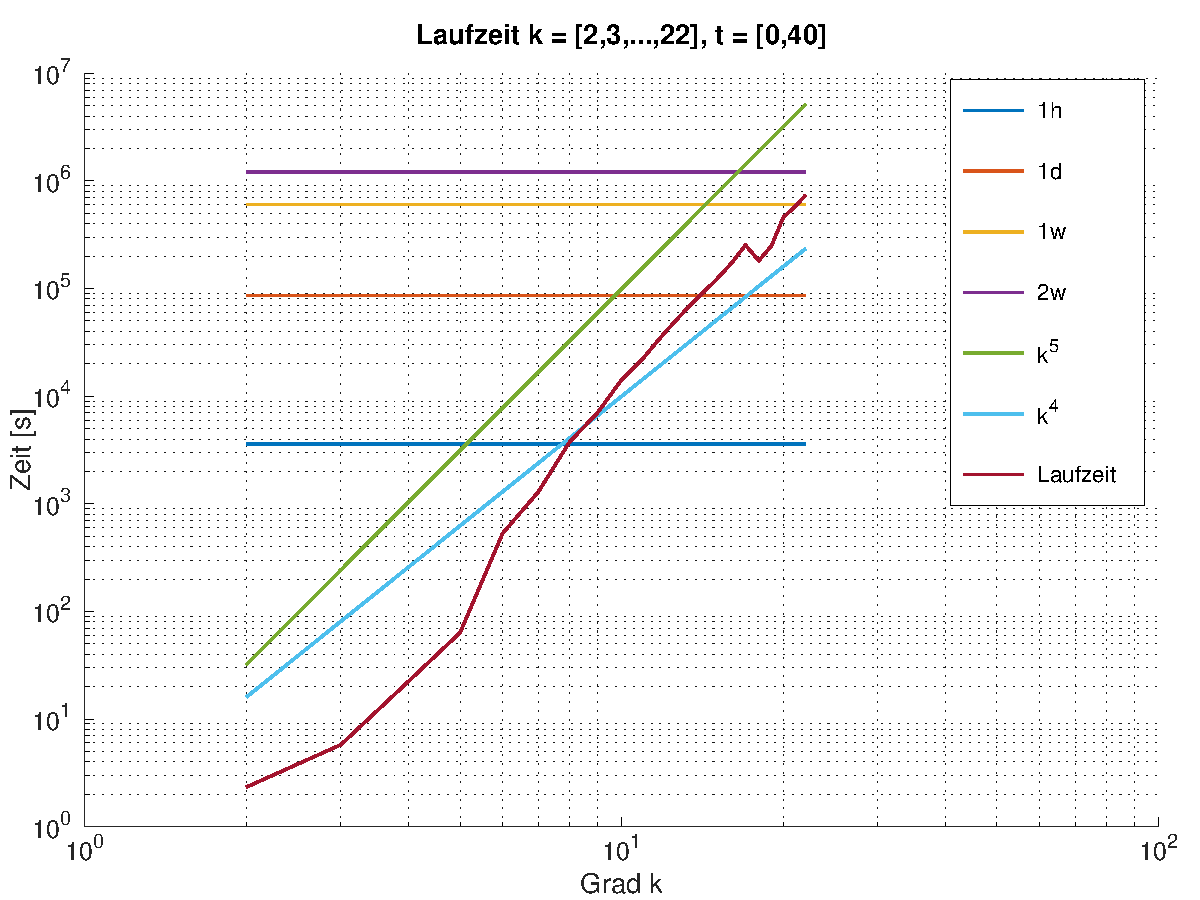
\includegraphics[width=0.49\linewidth]{lorenz2/03-images/timing_40}
	\caption{Laufzeit f"ur Berechnung von eines Lorenzsystems mit Grad $k$}
	\label{figure:lorenz2:timings}
\end{figure}

\begin{figure}
	\centering
	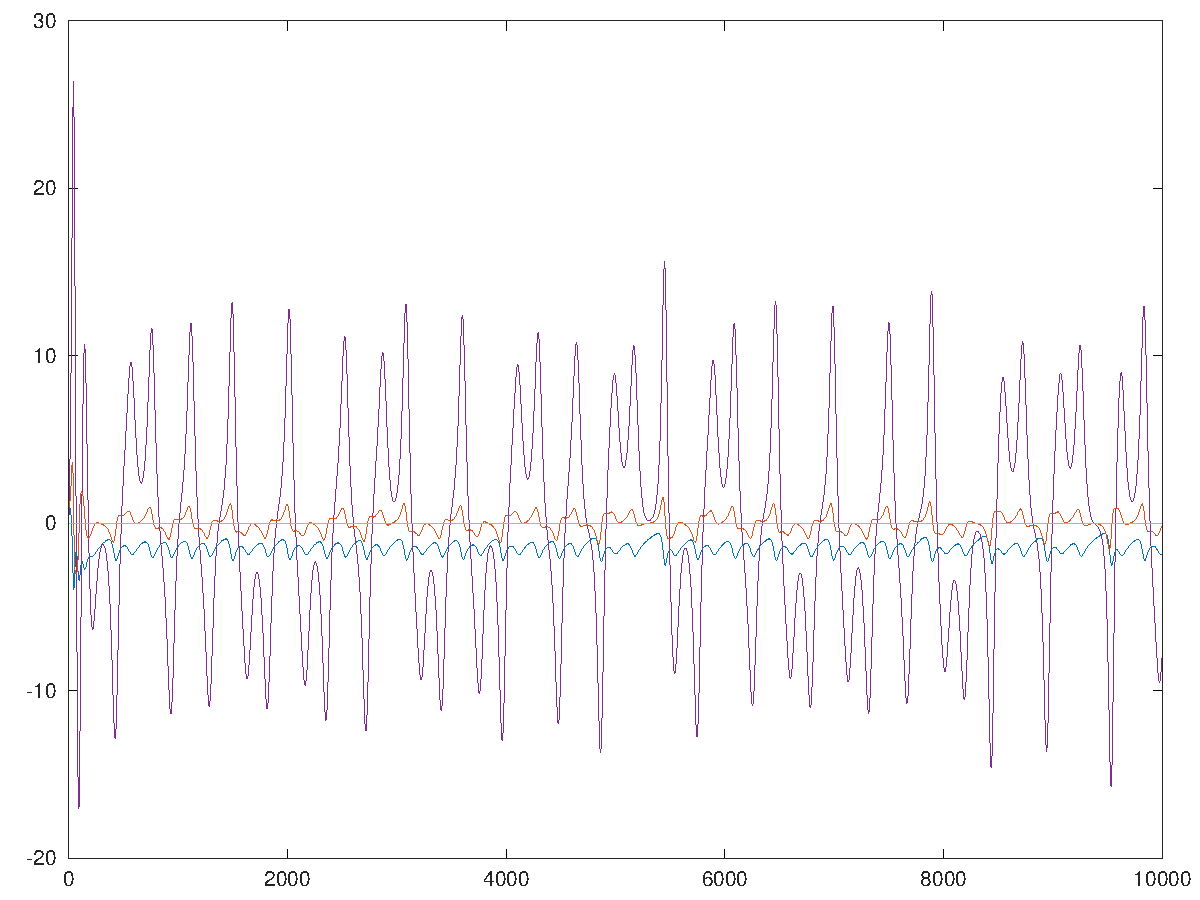
\includegraphics[width=0.49\linewidth]{{lorenz2/03-images/ord2.X}.pdf}
	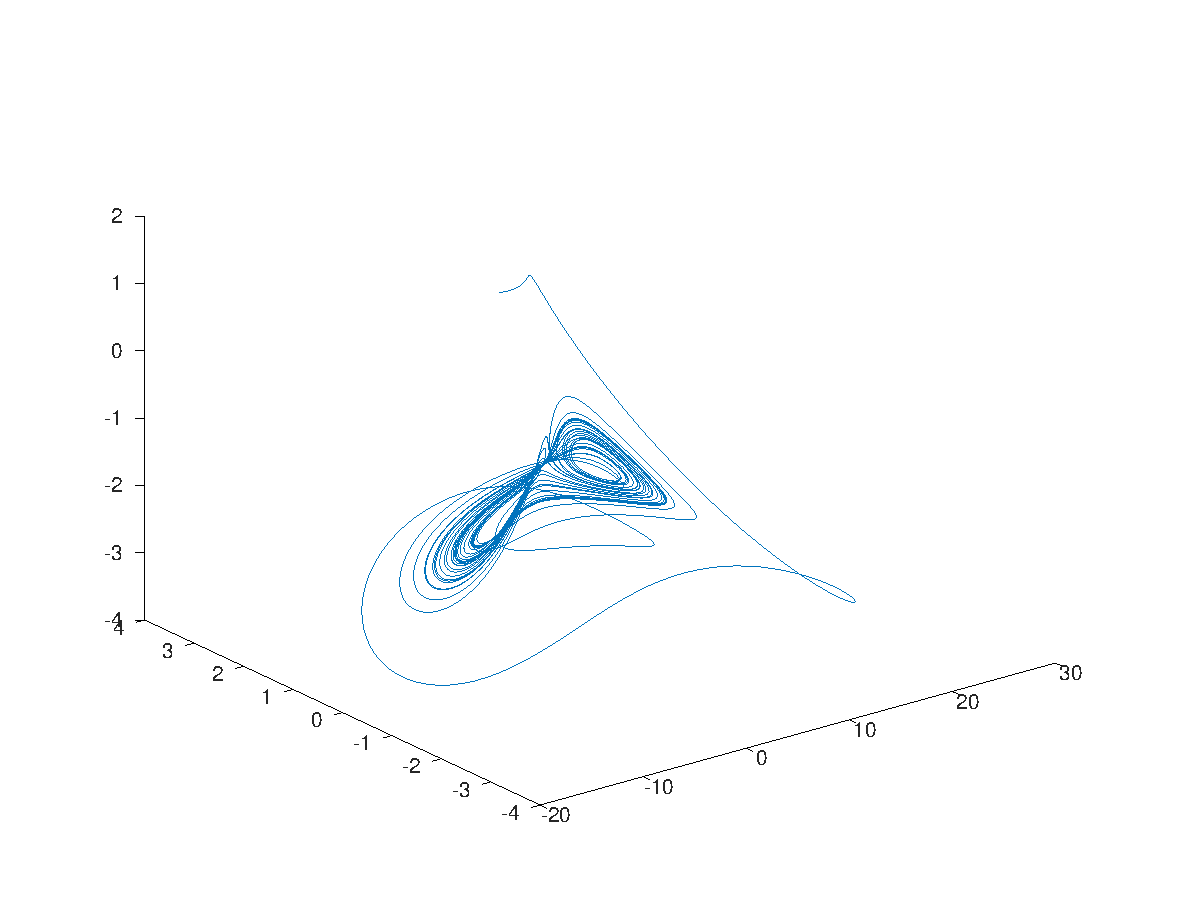
\includegraphics[width=0.49\linewidth]{{lorenz2/03-images/ord2.butterfly}.pdf}
	\caption{Lorenzssystem mit Grad 2}
	\label{figure:lorenz2:systemdeg2}
\end{figure}

\begin{figure}
	\centering
	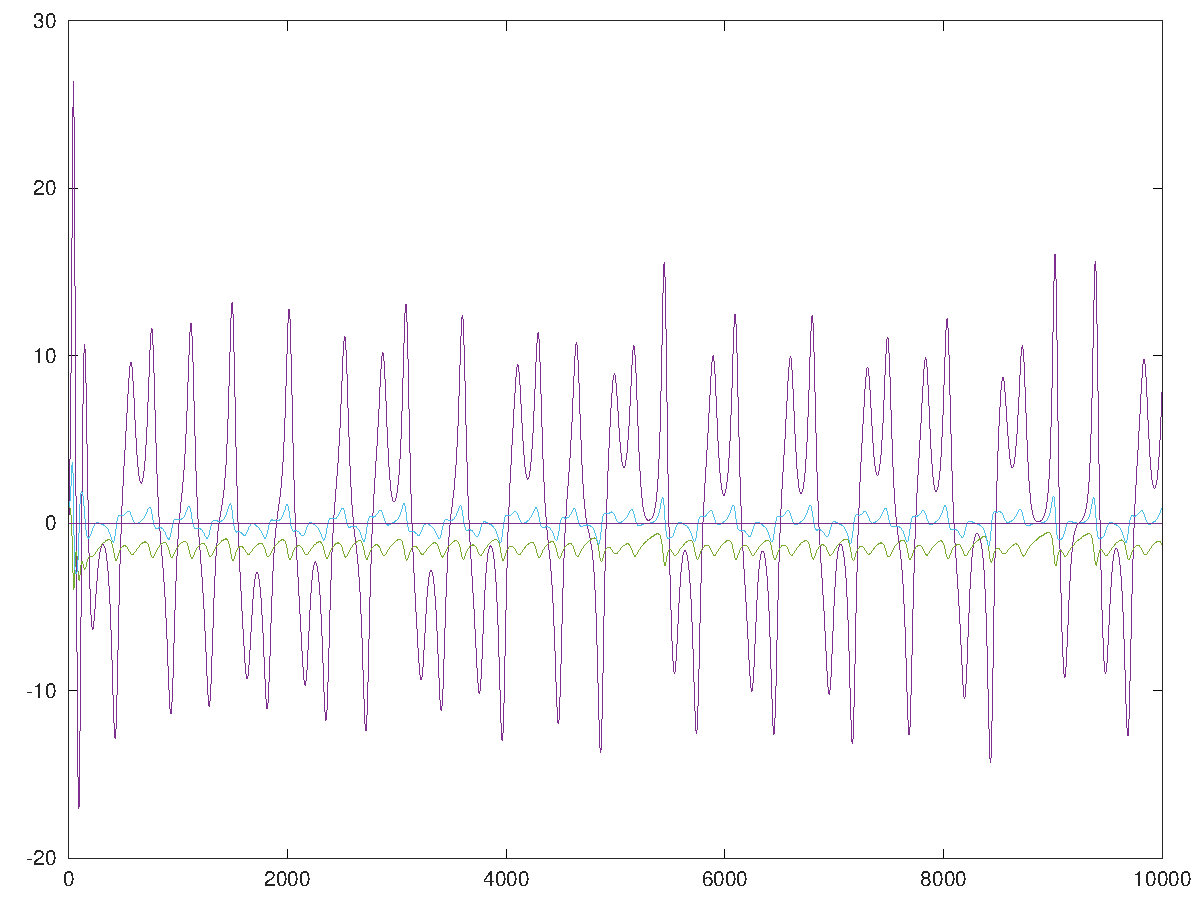
\includegraphics[width=0.49\linewidth]{{lorenz2/03-images/ord3.X}.pdf}
	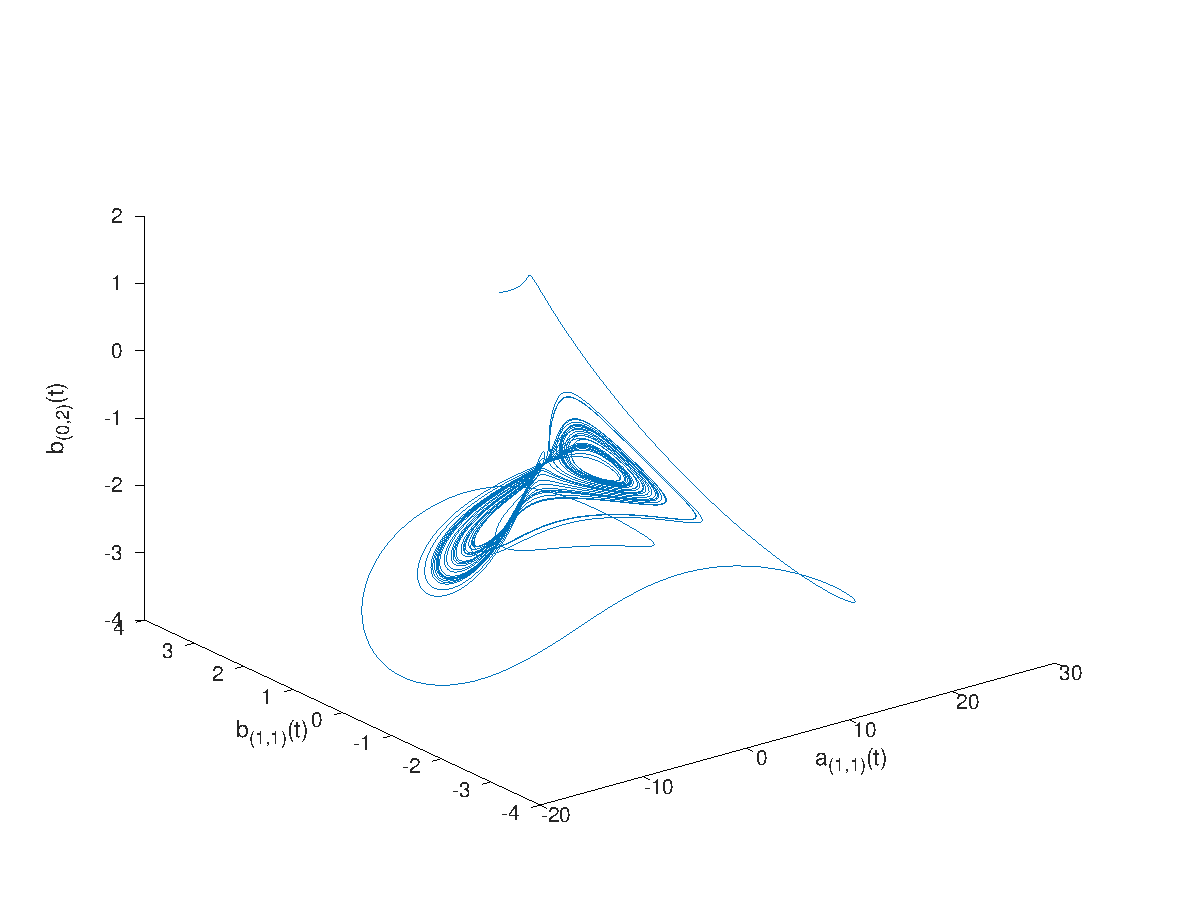
\includegraphics[width=0.49\linewidth]{{lorenz2/03-images/ord3.butterfly}.pdf}
	\caption{Lorenzssystem mit Grad 3}
	\label{figure:lorenz2:systemdeg3}
\end{figure}

\begin{figure}
	\centering
	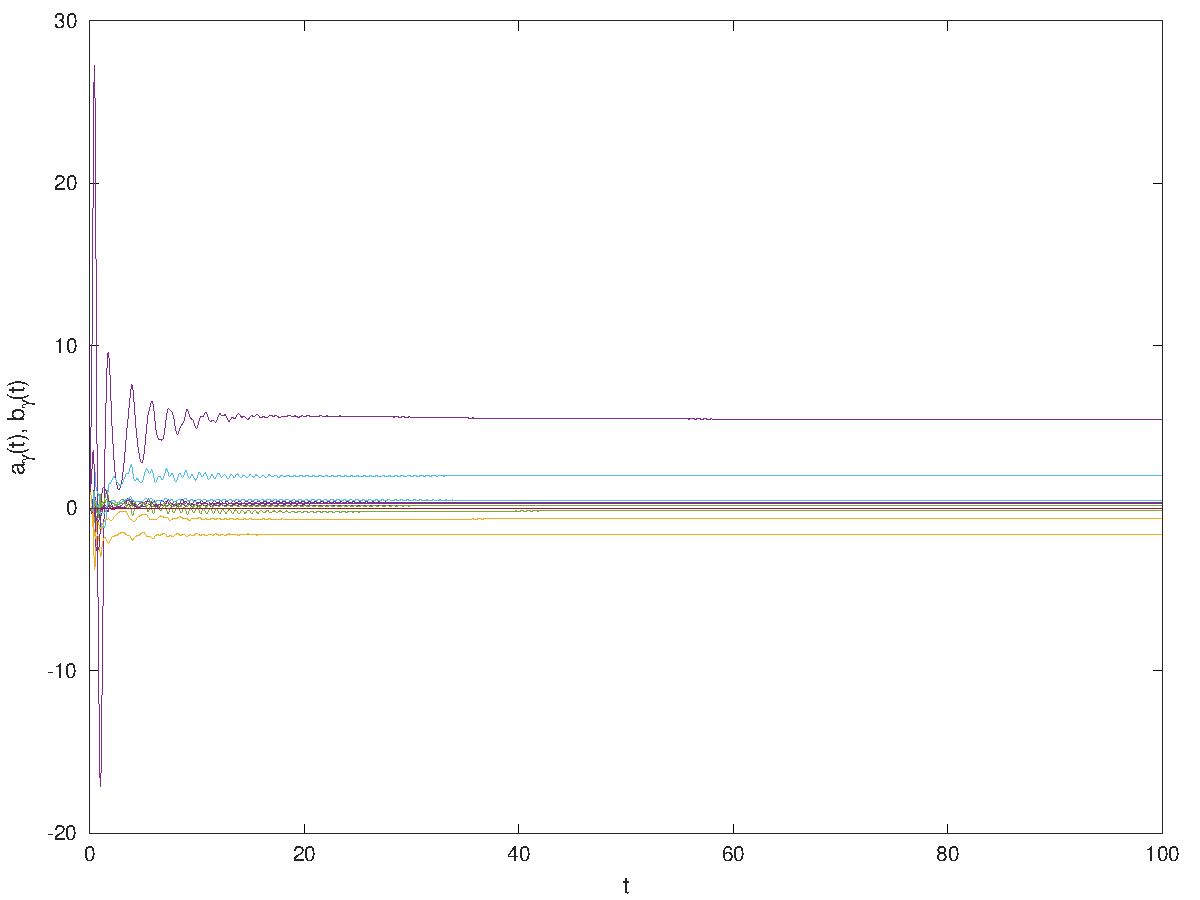
\includegraphics[width=0.49\linewidth]{{lorenz2/03-images/ord4.X}.pdf}
	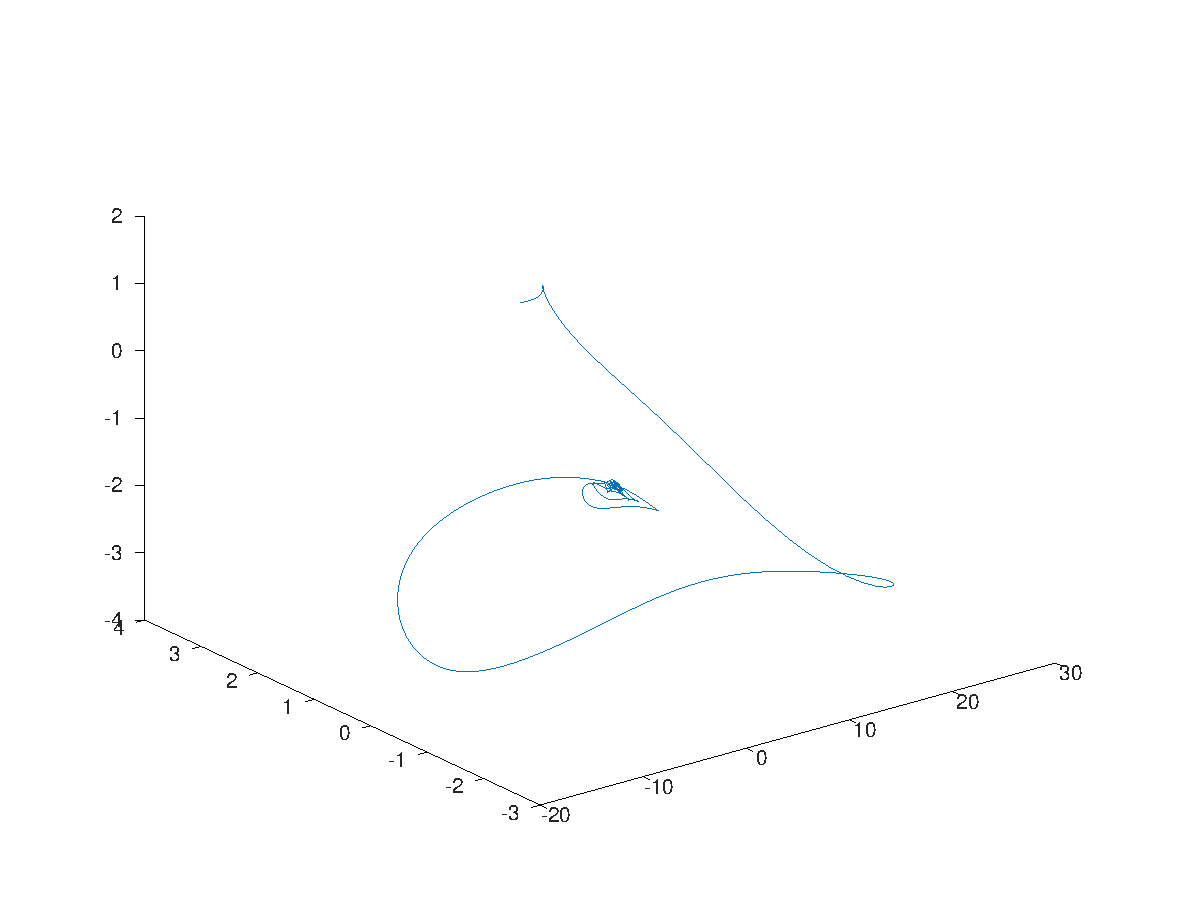
\includegraphics[width=0.49\linewidth]{{lorenz2/03-images/ord4.butterfly}.pdf}
	\caption{Lorenzssystem mit Grad 4}
	\label{figure:lorenz2:systemdeg4}
\end{figure}

\begin{figure}
	\centering
	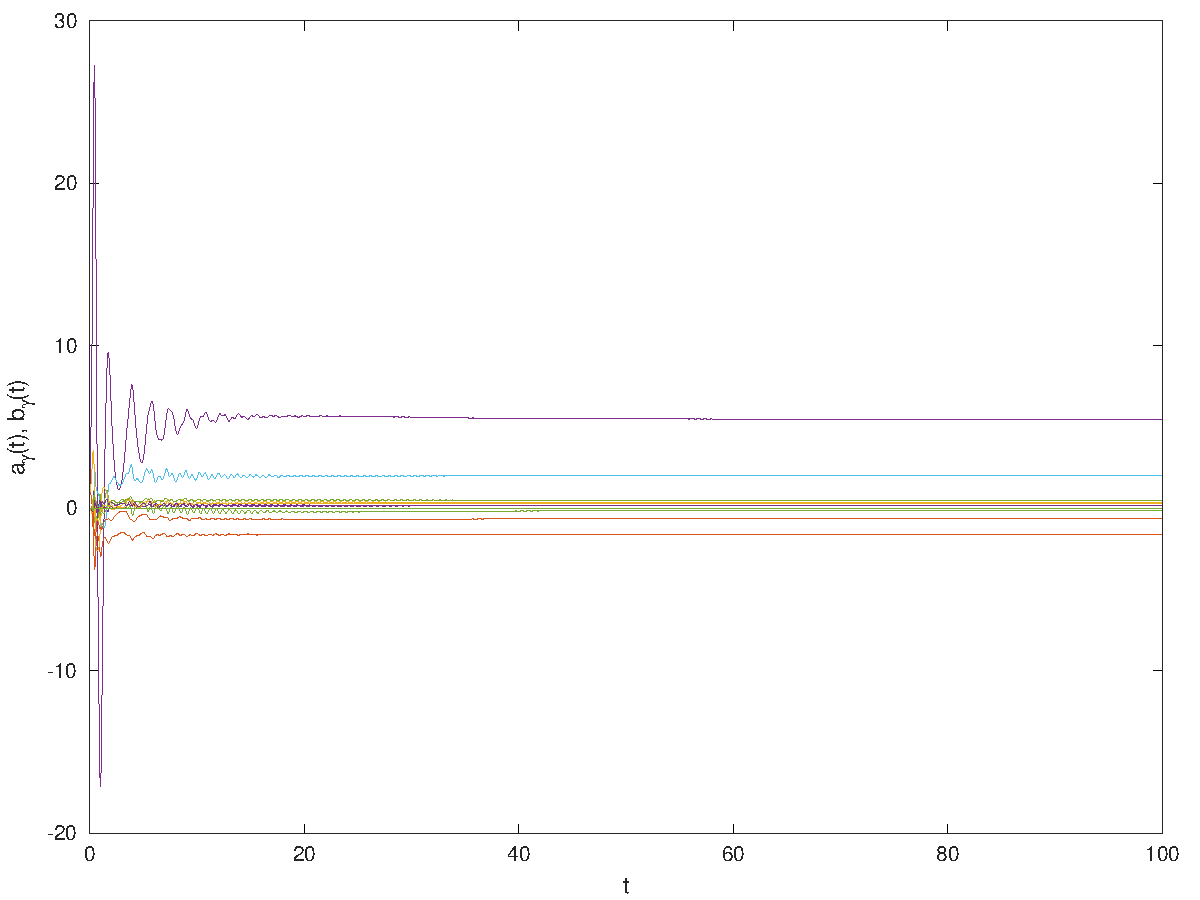
\includegraphics[width=0.49\linewidth]{{lorenz2/03-images/ord5.X}.pdf}
	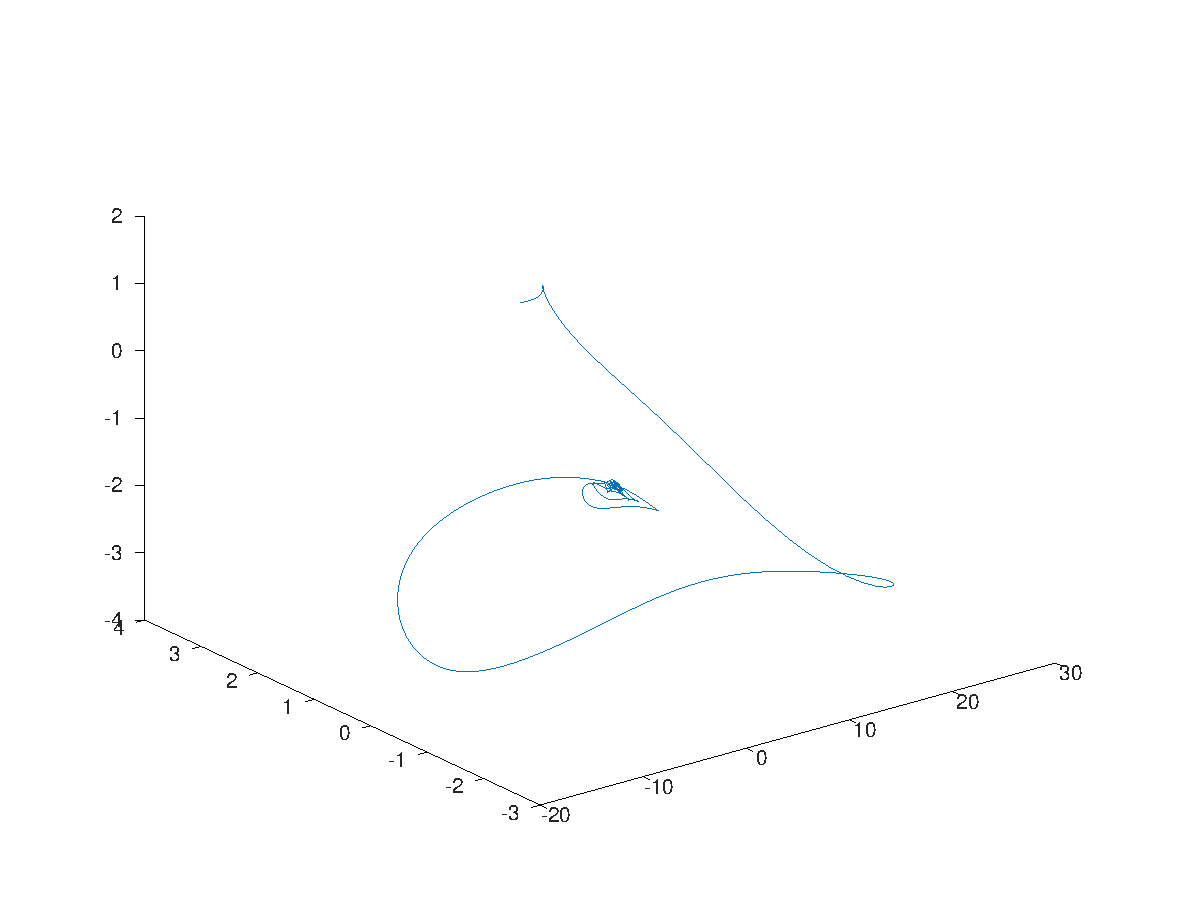
\includegraphics[width=0.49\linewidth]{{lorenz2/03-images/ord5.butterfly}.pdf}
	\caption{Lorenzssystem mit Grad 5}
	\label{figure:lorenz2:systemdeg5}
\end{figure}

\begin{figure}
	\centering
	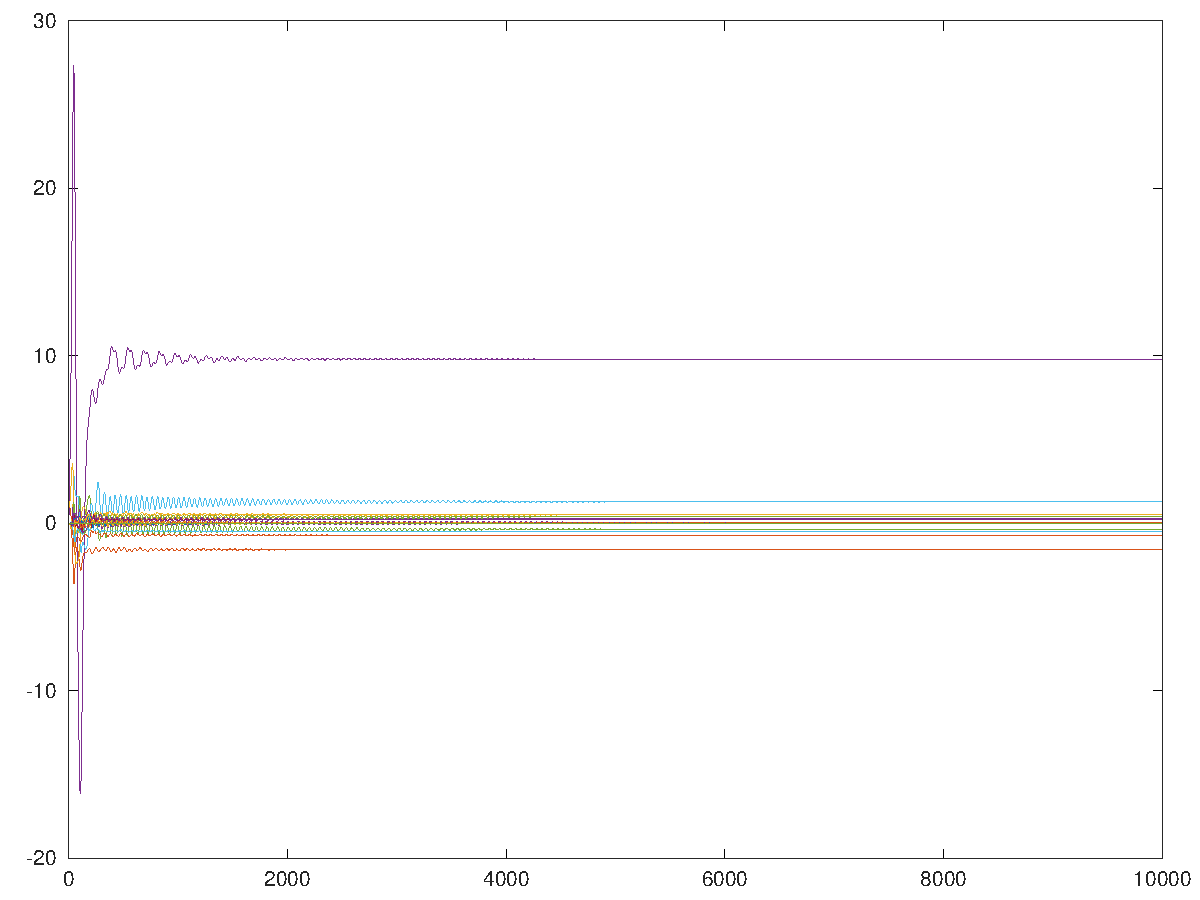
\includegraphics[width=0.49\linewidth]{{lorenz2/03-images/ord6.X}.pdf}
	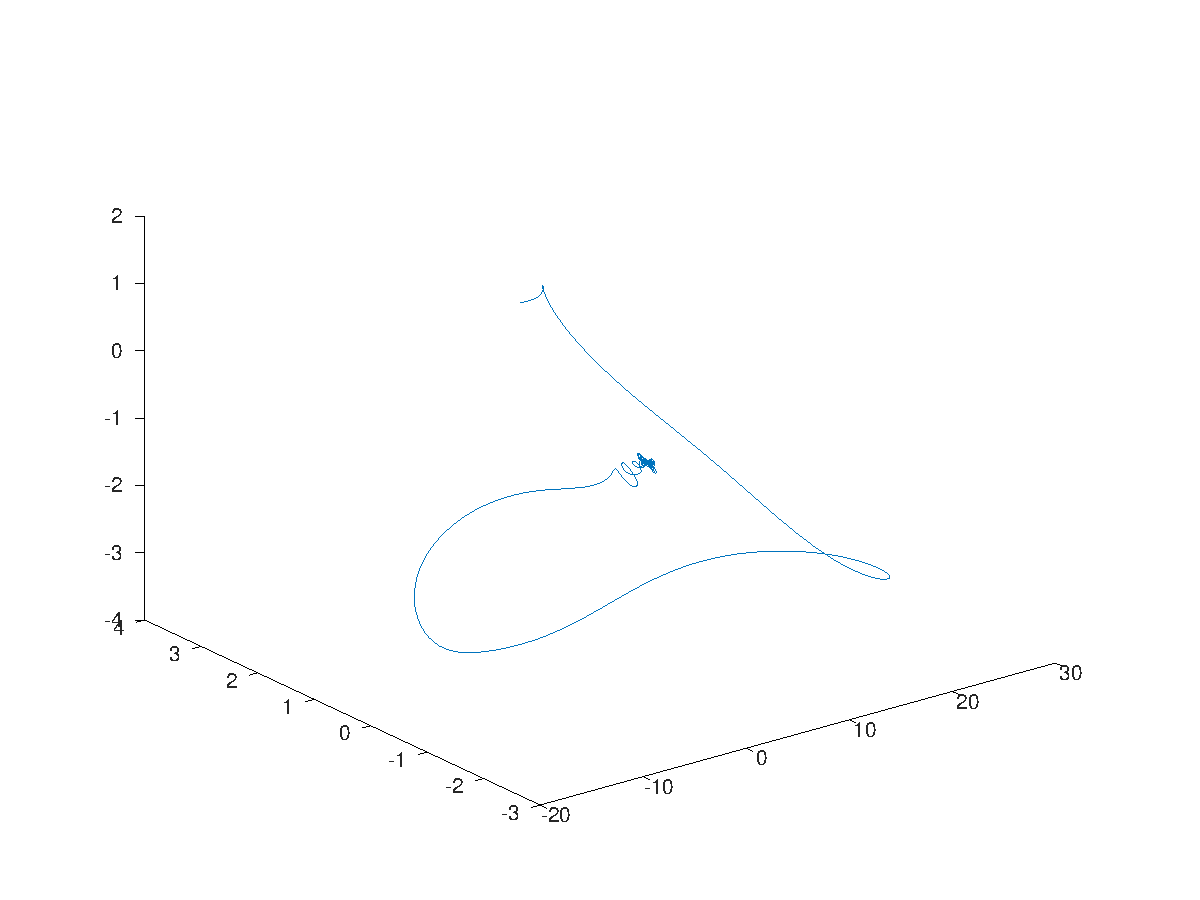
\includegraphics[width=0.49\linewidth]{{lorenz2/03-images/ord6.butterfly}.pdf}
	\caption{Lorenzssystem mit Grad 6}
	\label{figure:lorenz2:systemdeg6}
\end{figure}

\begin{figure}
	\centering
	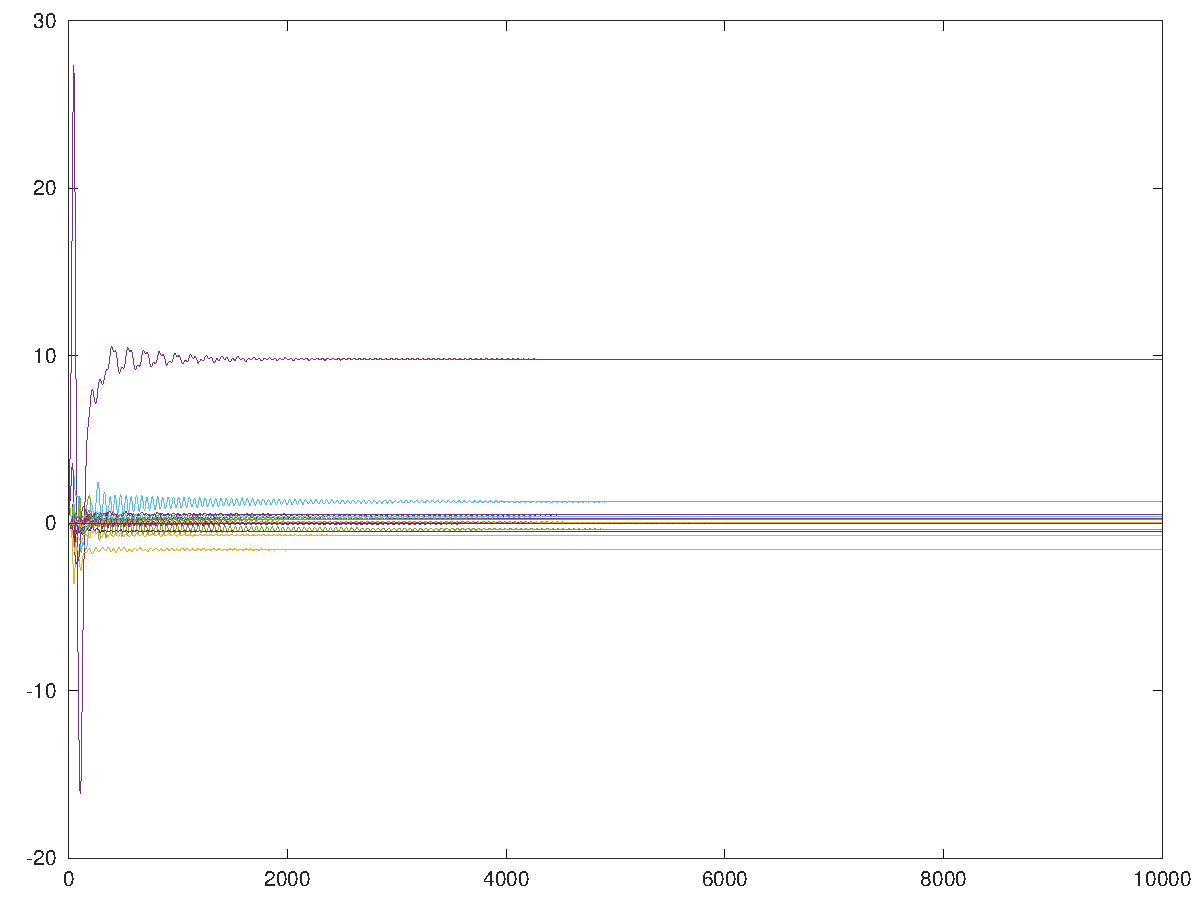
\includegraphics[width=0.49\linewidth]{{lorenz2/03-images/ord7.X}.pdf}
	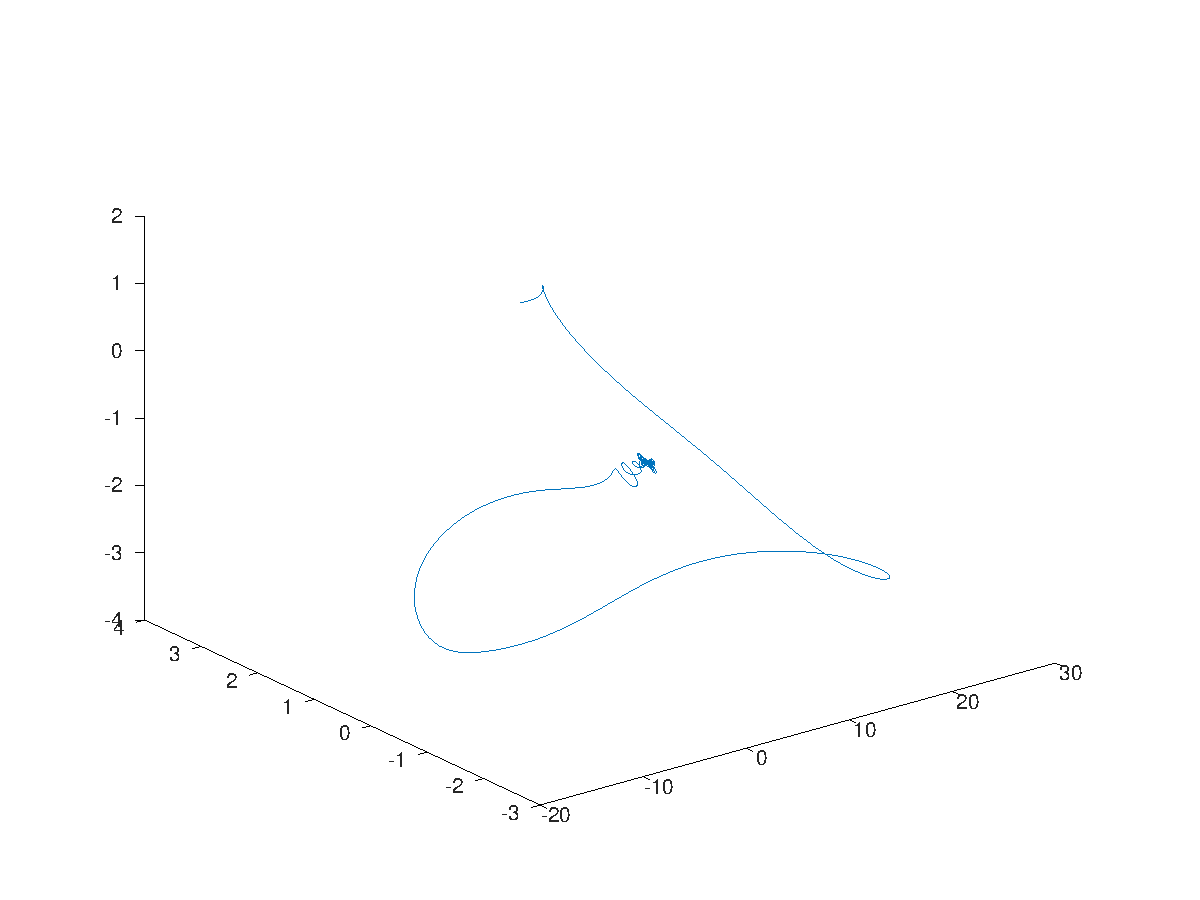
\includegraphics[width=0.49\linewidth]{{lorenz2/03-images/ord7.butterfly}.pdf}
	\caption{Lorenzssystem mit Grad 7}
	\label{figure:lorenz2:systemdeg7}
\end{figure}

\begin{figure}
	\centering
	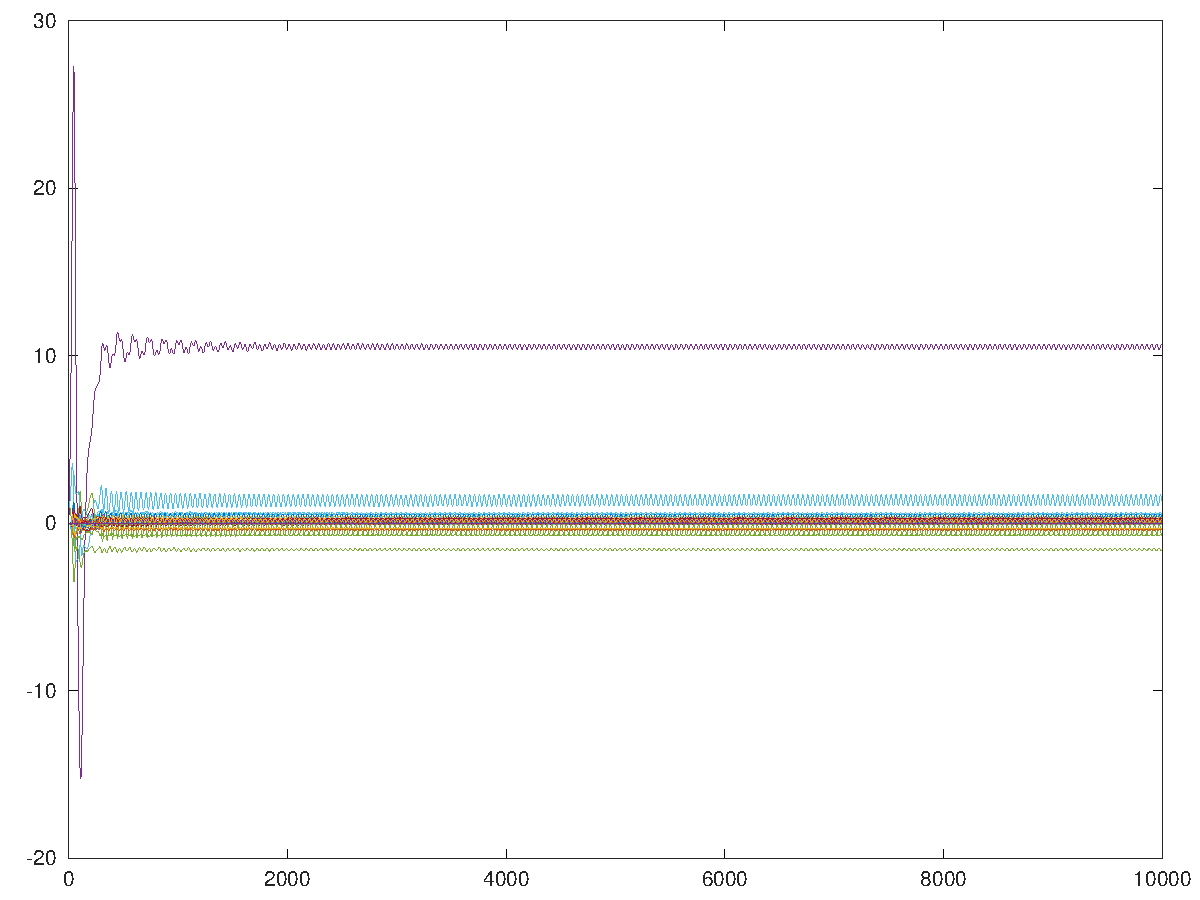
\includegraphics[width=0.49\linewidth]{{lorenz2/03-images/ord8.X}.pdf}
	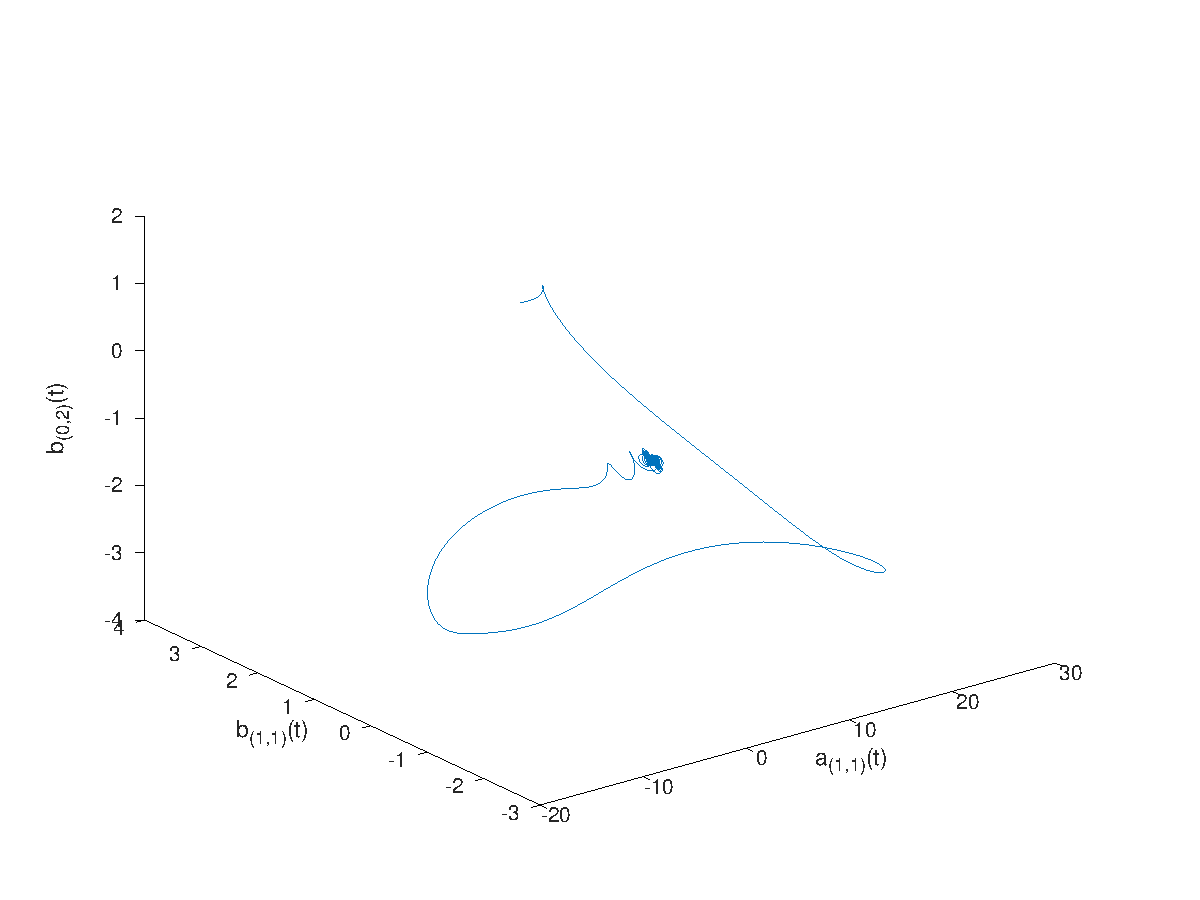
\includegraphics[width=0.49\linewidth]{{lorenz2/03-images/ord8.butterfly}.pdf}
	\caption{Lorenzssystem mit Grad 8}
	\label{figure:lorenz2:systemdeg8}
\end{figure}

\begin{figure}
	\centering
	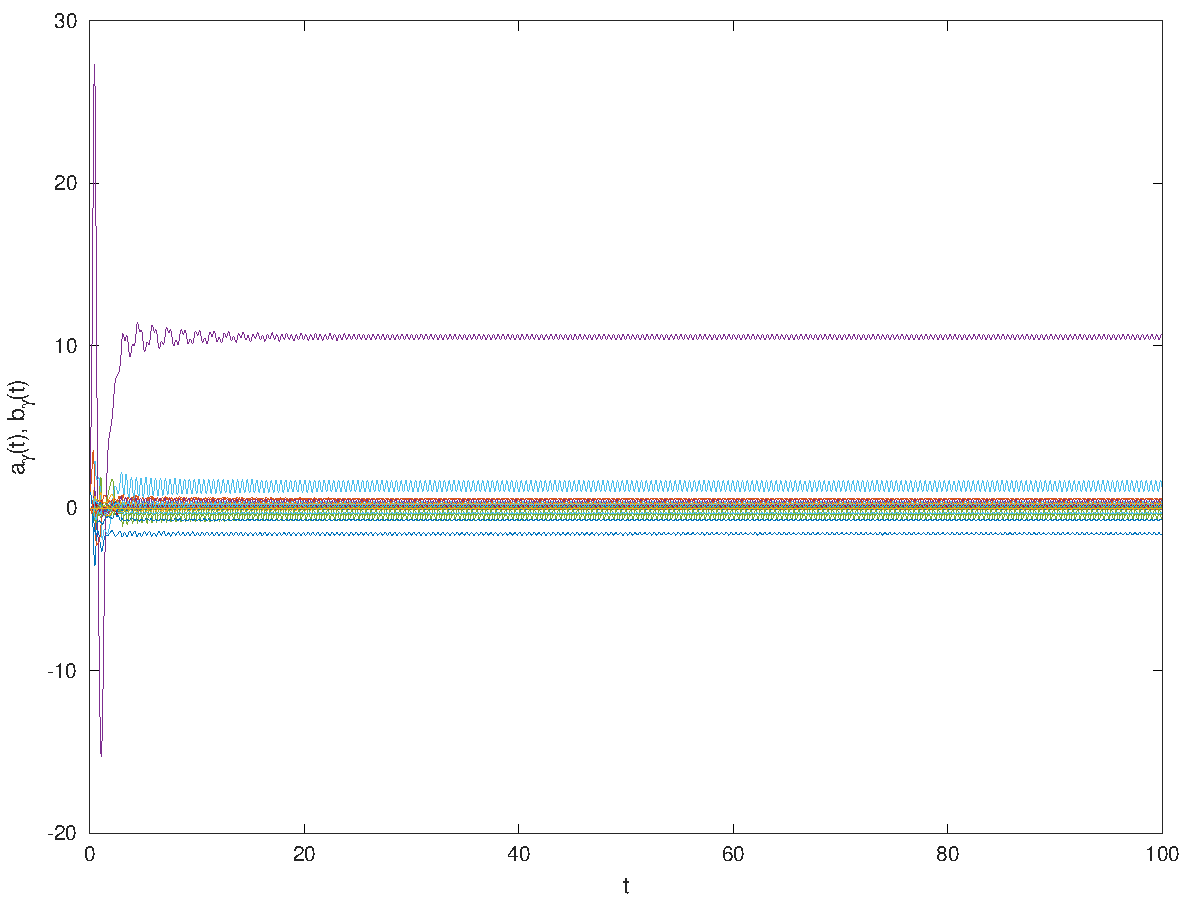
\includegraphics[width=0.49\linewidth]{{lorenz2/03-images/ord9.X}.pdf}
	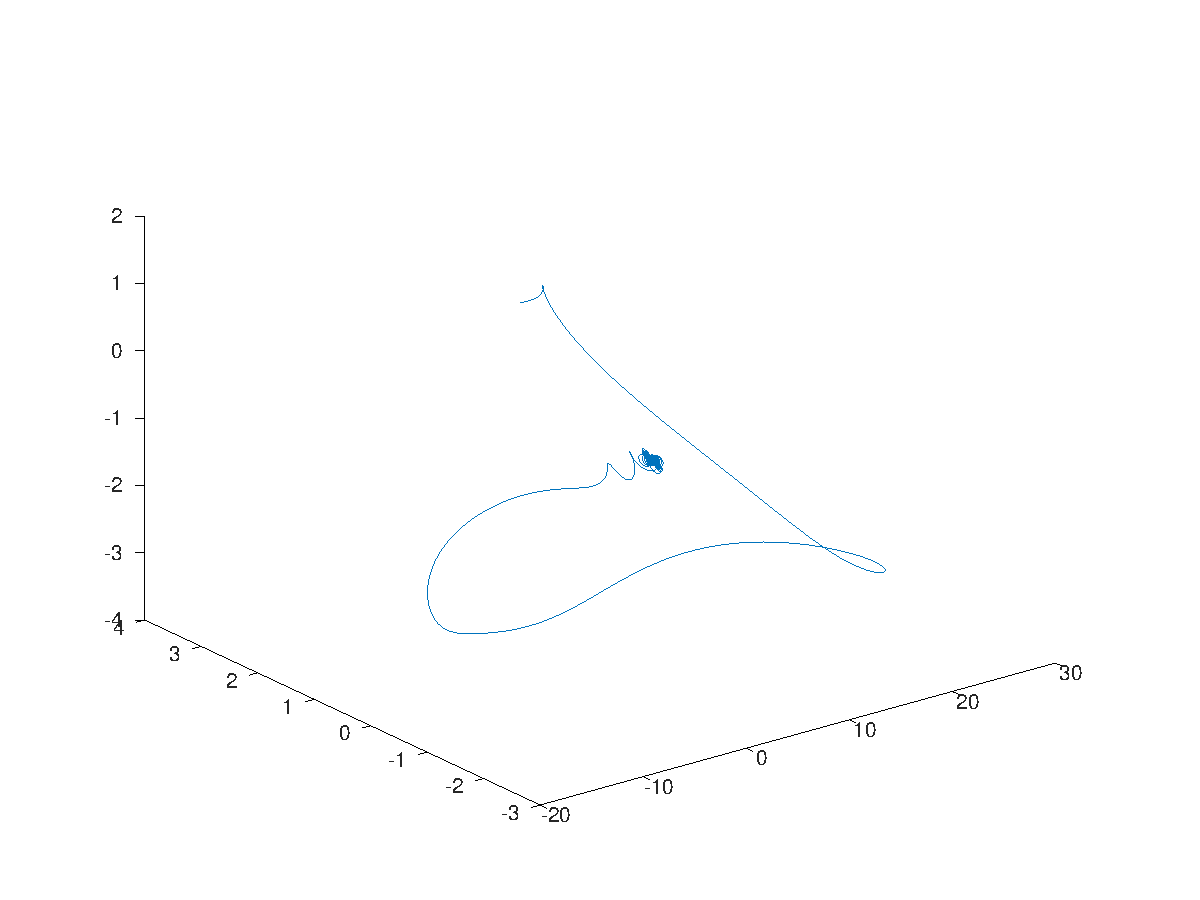
\includegraphics[width=0.49\linewidth]{{lorenz2/03-images/ord9.butterfly}.pdf}
	\caption{Lorenzssystem mit Grad 9}
	\label{figure:lorenz2:systemdeg9}
\end{figure}

\begin{figure}
	\centering
	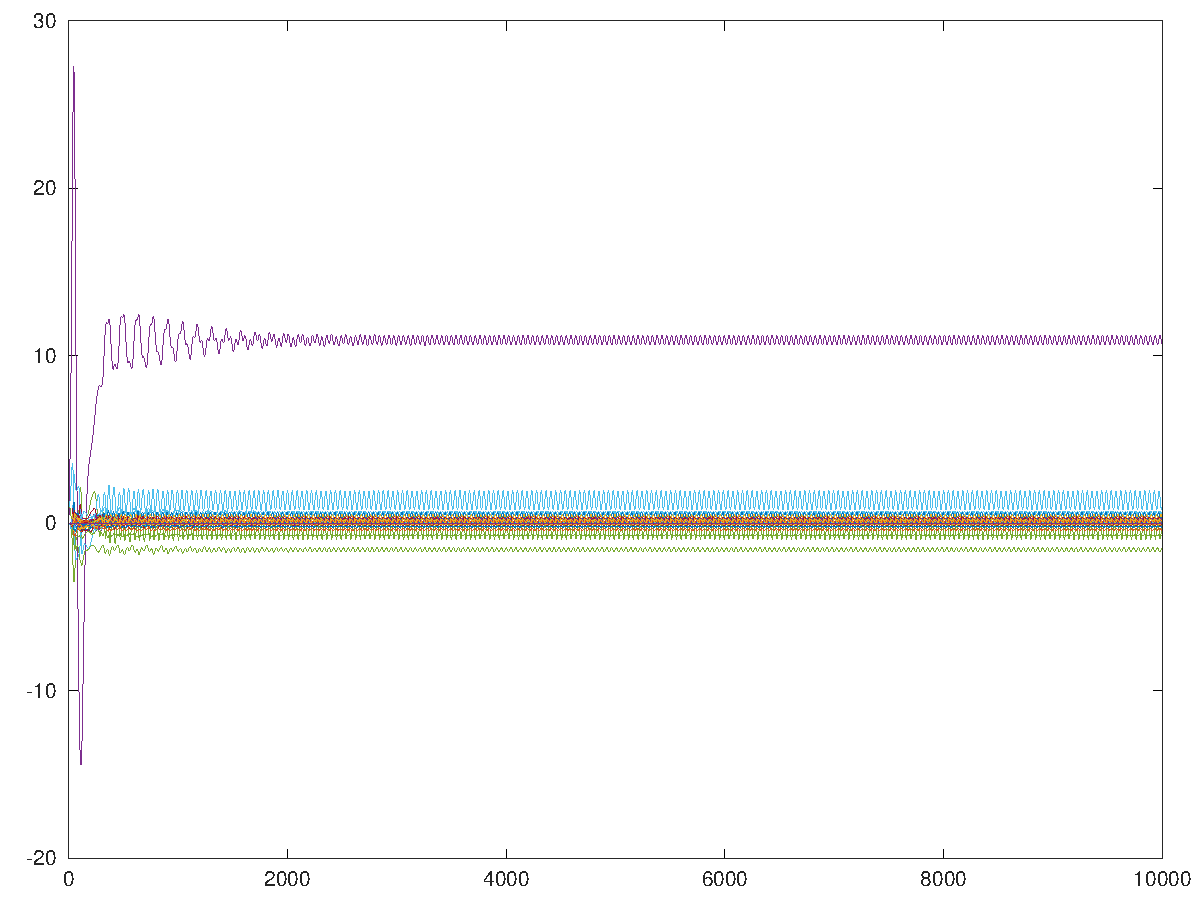
\includegraphics[width=0.49\linewidth]{{lorenz2/03-images/ord10.X}.pdf}
	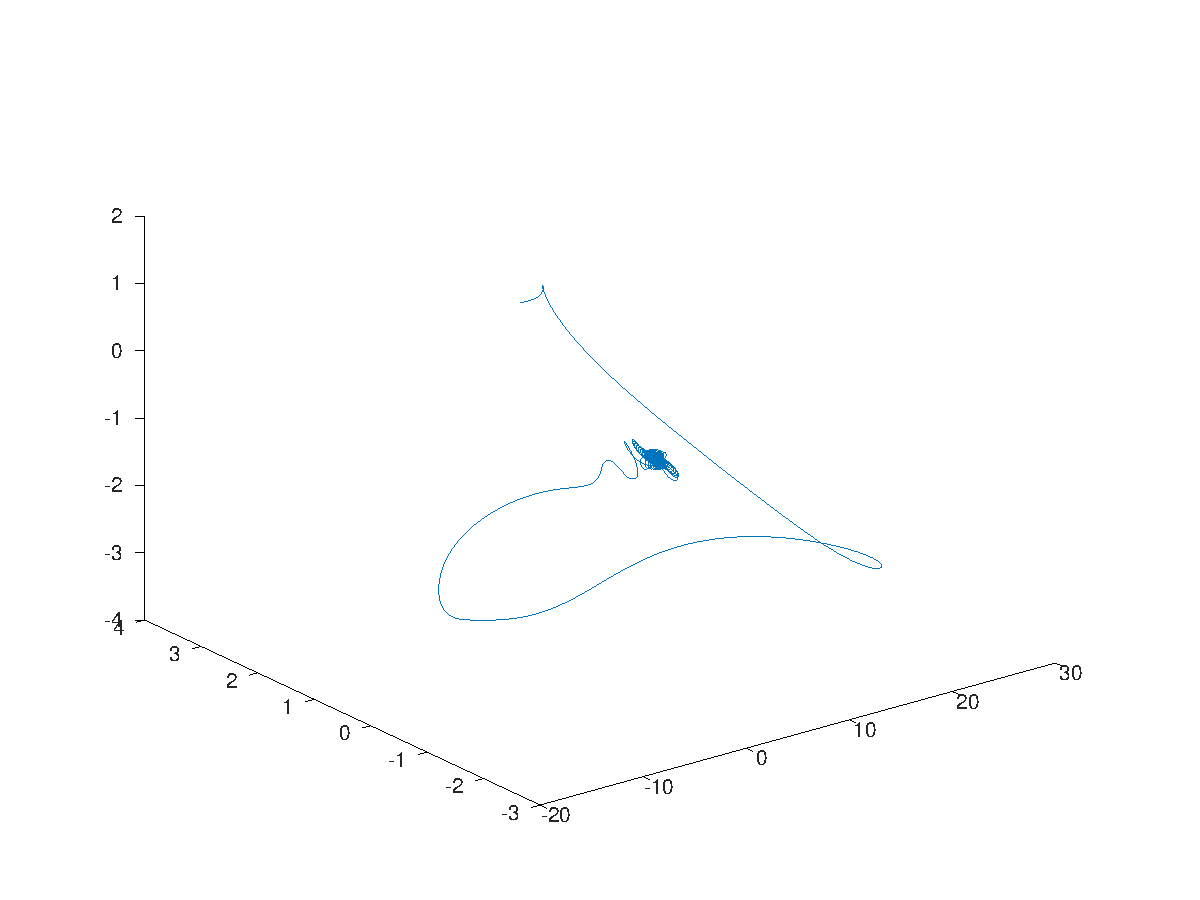
\includegraphics[width=0.49\linewidth]{{lorenz2/03-images/ord10.butterfly}.pdf}
	\caption{Lorenzssystem mit Grad 10, $t = [0,100]$}
	\label{figure:lorenz2:systemdeg10}
\end{figure}

\begin{figure}
	\centering
	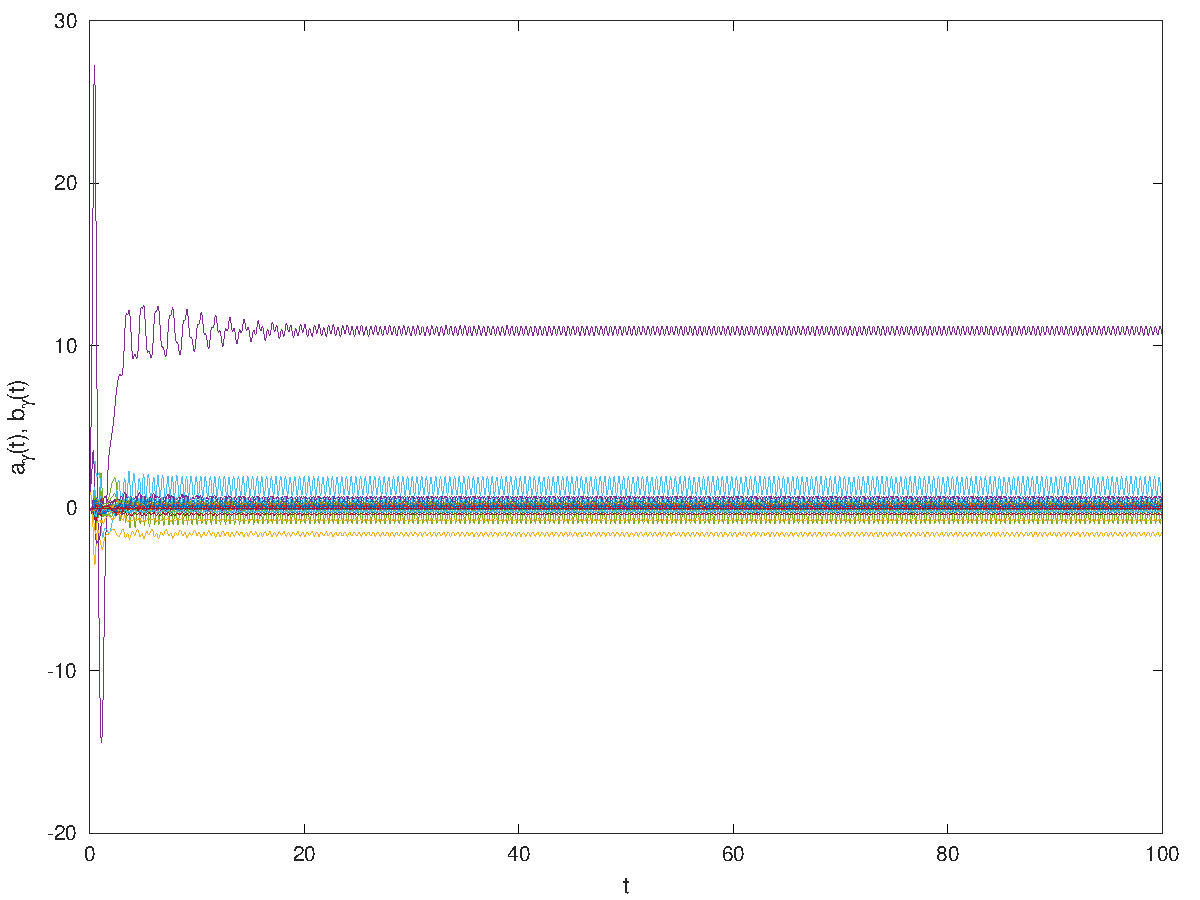
\includegraphics[width=0.49\linewidth]{{lorenz2/03-images/ord11.X}.pdf}
	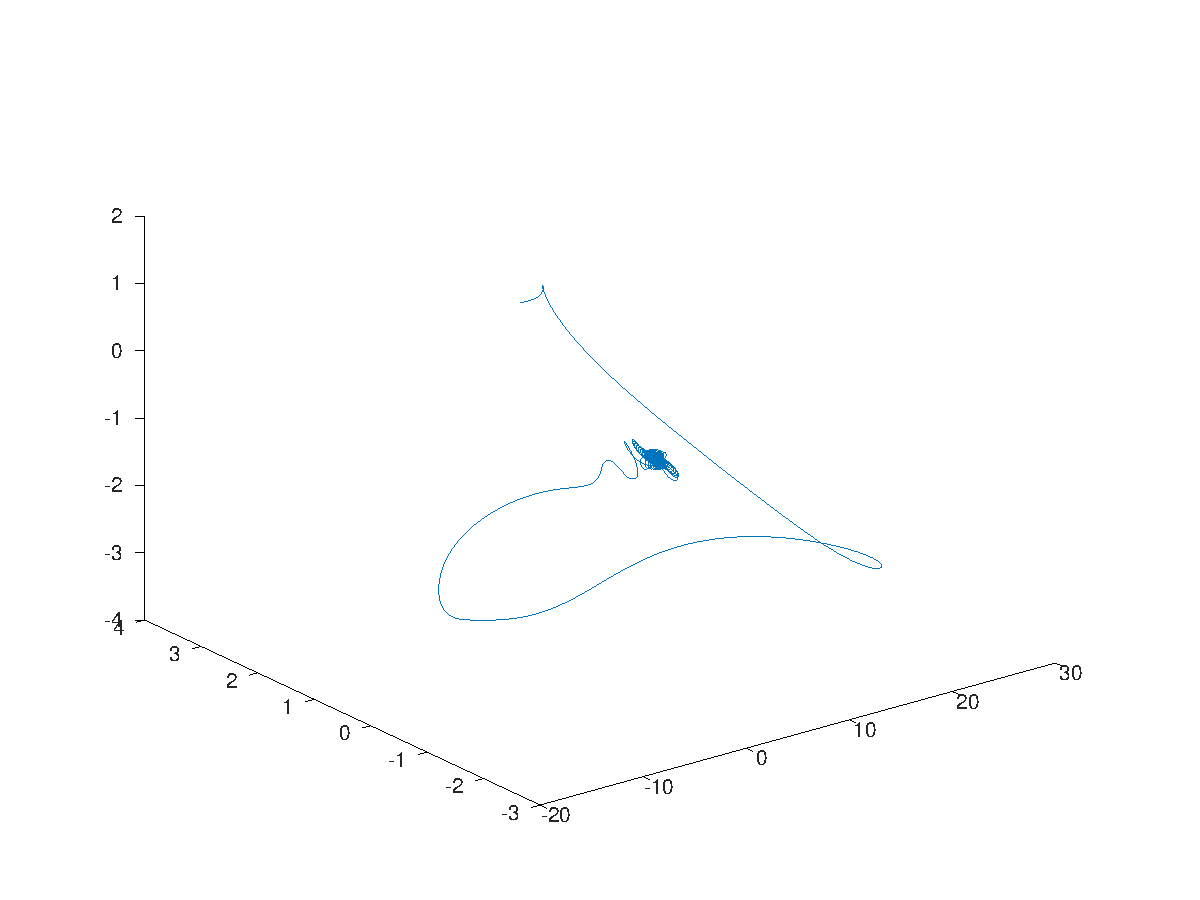
\includegraphics[width=0.49\linewidth]{{lorenz2/03-images/ord11.butterfly}.pdf}
	\caption{Lorenzssystem mit Grad 11, $t = [0,100]$}
	\label{figure:lorenz2:systemdeg11}
\end{figure}

\begin{figure}
	\centering
	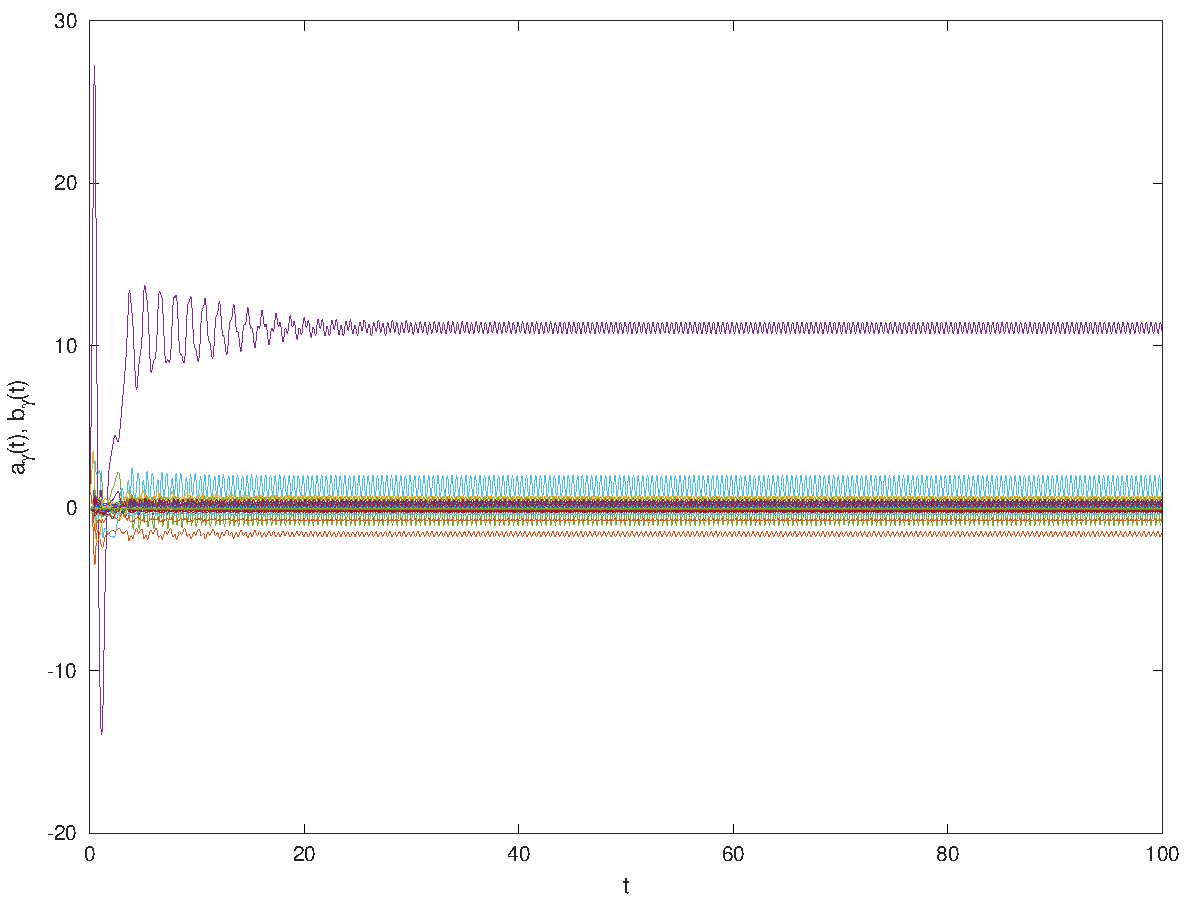
\includegraphics[width=0.49\linewidth]{{lorenz2/03-images/ord12.X}.pdf}
	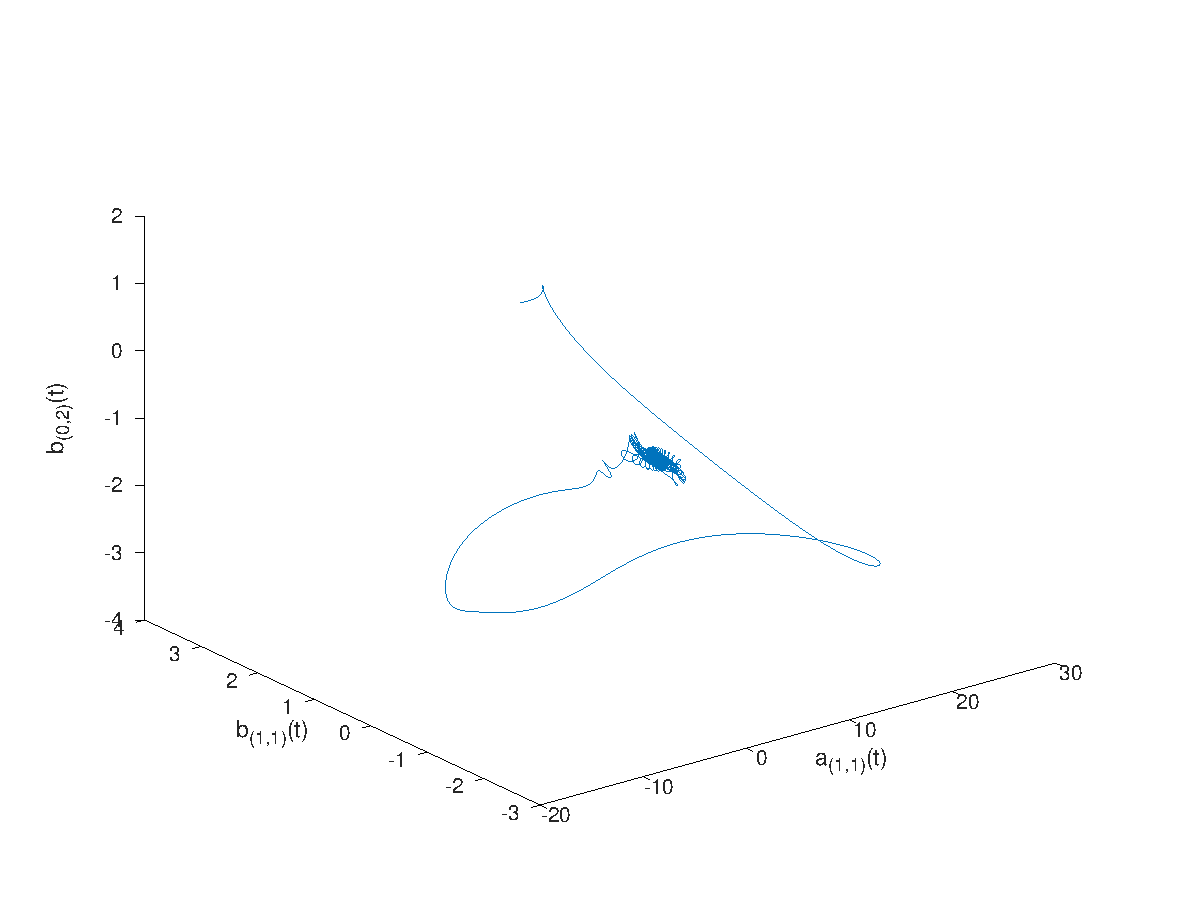
\includegraphics[width=0.49\linewidth]{{lorenz2/03-images/ord12.butterfly}.pdf}
	\caption{Lorenzssystem mit Grad 12, $t = [0,100]$}
	\label{figure:lorenz2:systemdeg12}
\end{figure}

\begin{figure}
	\centering
	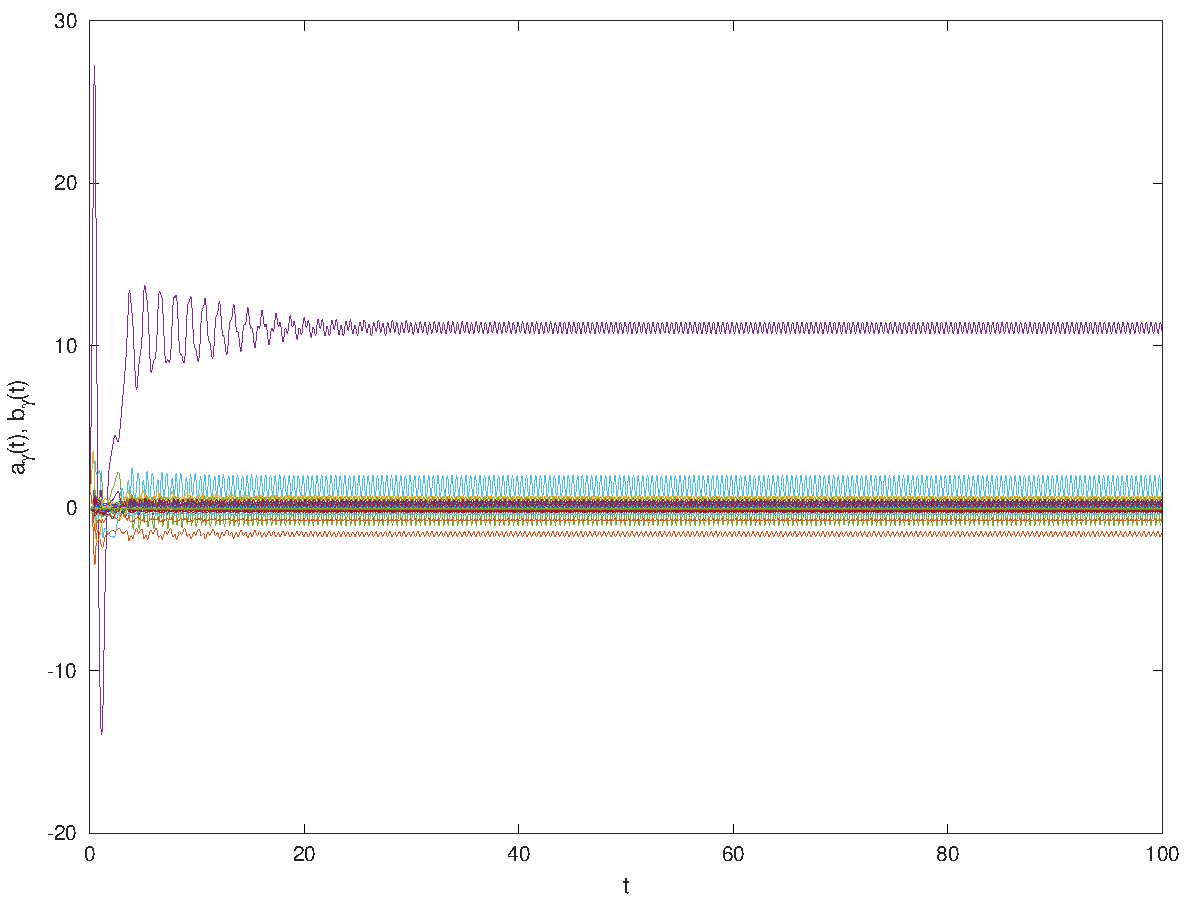
\includegraphics[width=0.49\linewidth]{{lorenz2/03-images/ord13.X}.pdf}
	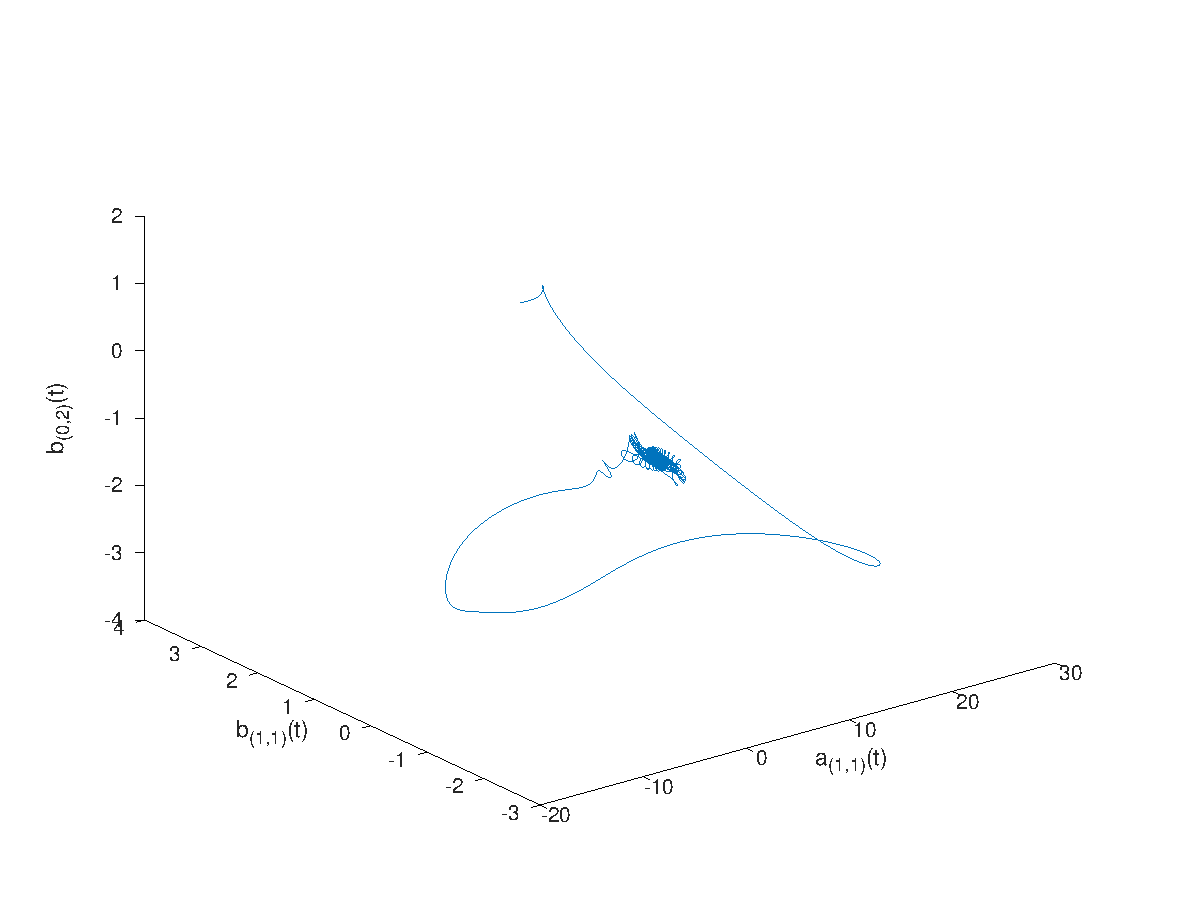
\includegraphics[width=0.49\linewidth]{{lorenz2/03-images/ord13.butterfly}.pdf}
	\caption{Lorenzssystem mit Grad 13, $t = [0,100]$}
	\label{figure:lorenz2:systemdeg13}
\end{figure}

\begin{figure}
	\centering
	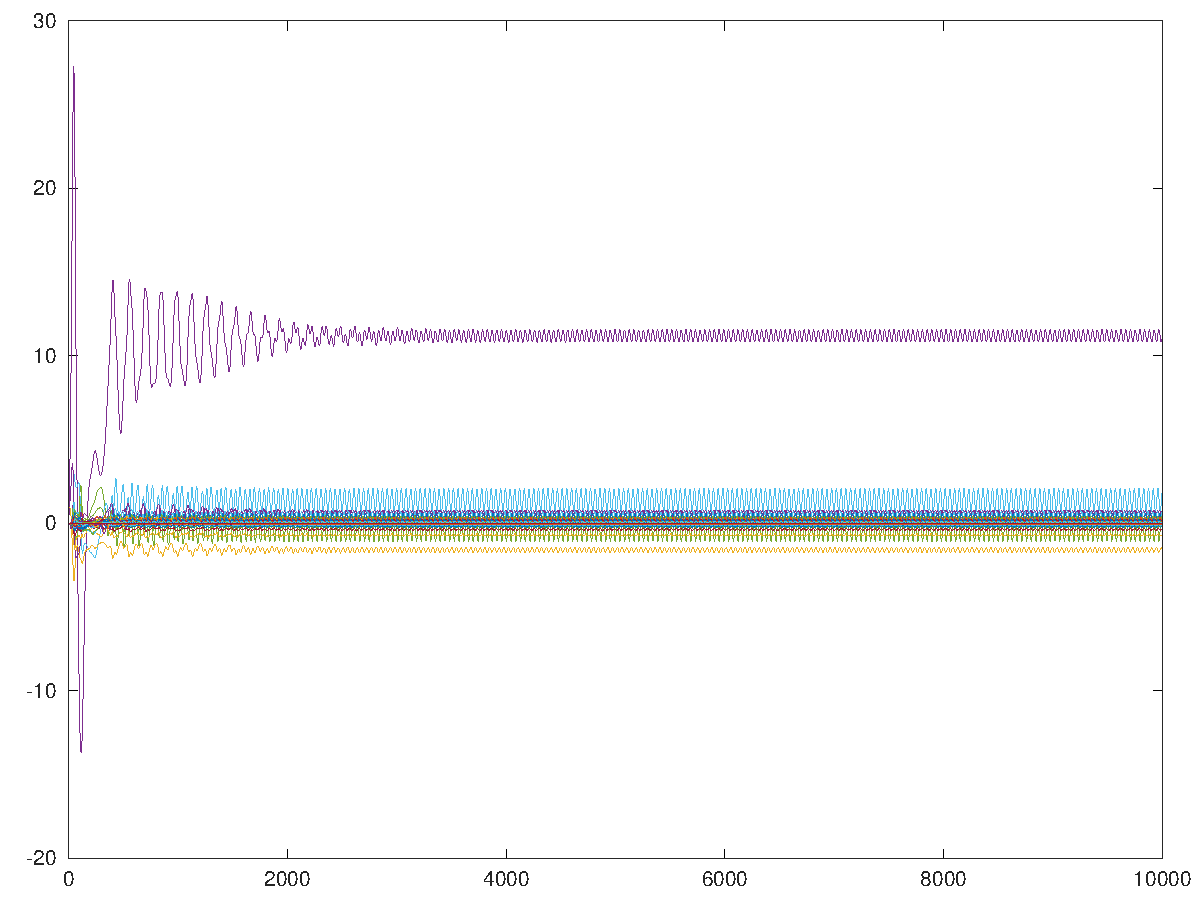
\includegraphics[width=0.49\linewidth]{{lorenz2/03-images/ord14.X}.pdf}
	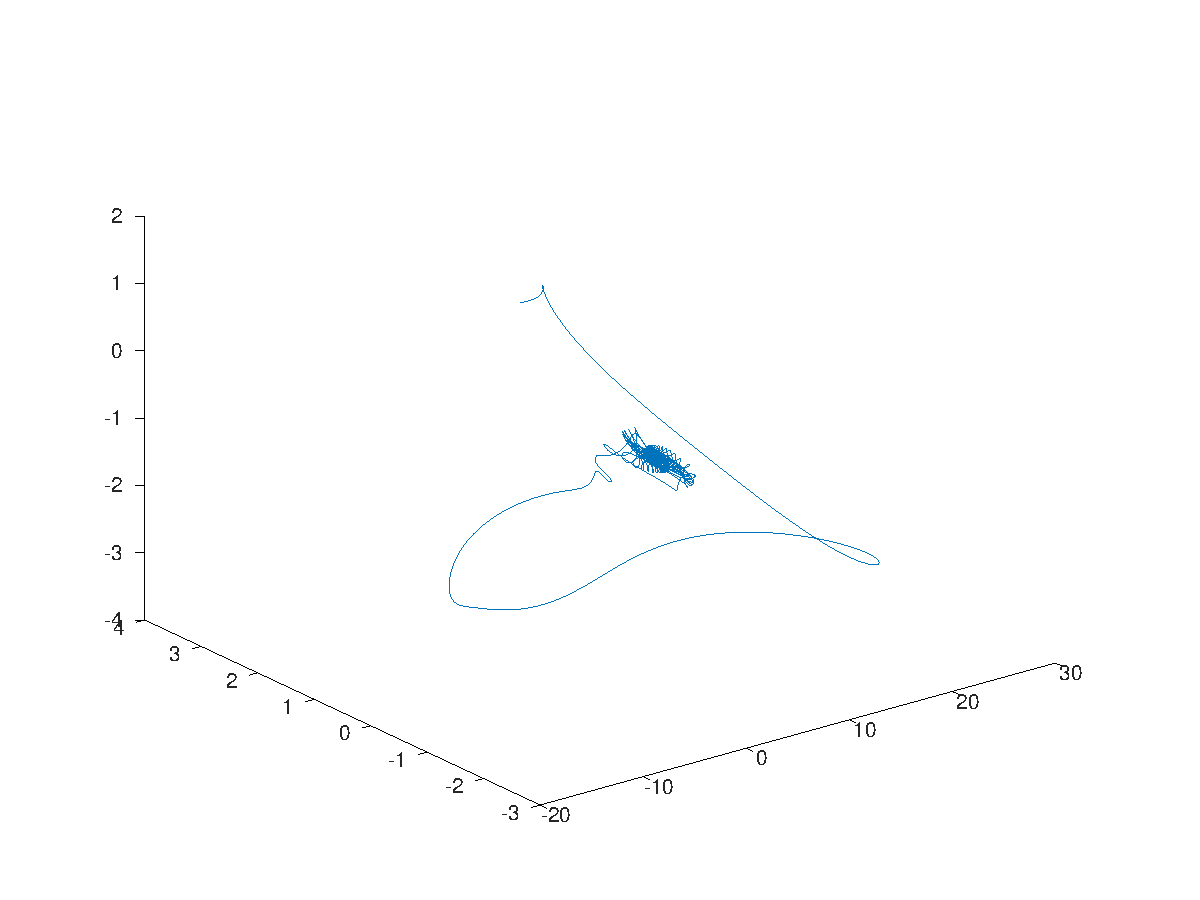
\includegraphics[width=0.49\linewidth]{{lorenz2/03-images/ord14.butterfly}.pdf}
	\caption{Lorenzssystem mit Grad 14, $t = [0,100]$}
	\label{figure:lorenz2:systemdeg14}
\end{figure}

\begin{figure}
	\centering
	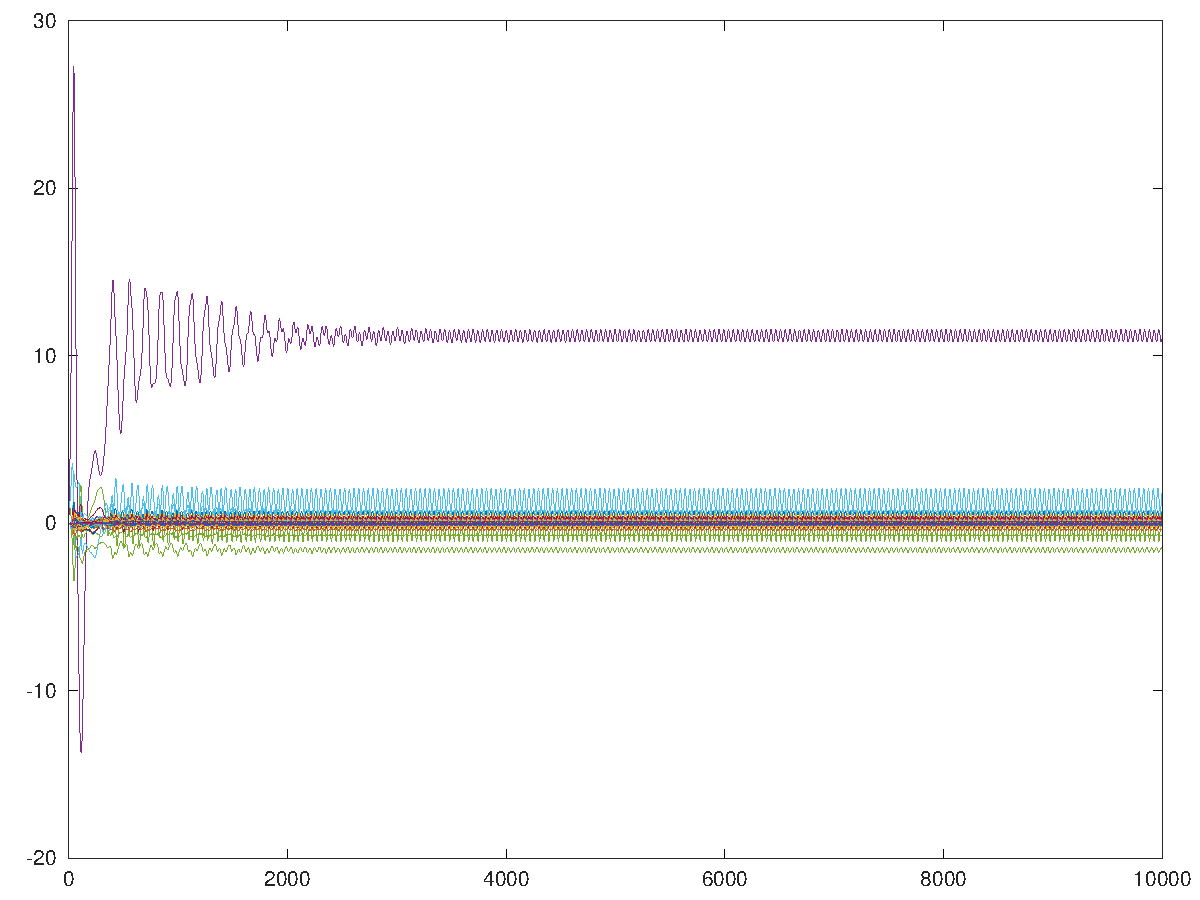
\includegraphics[width=0.49\linewidth]{{lorenz2/03-images/ord15.X}.pdf}
	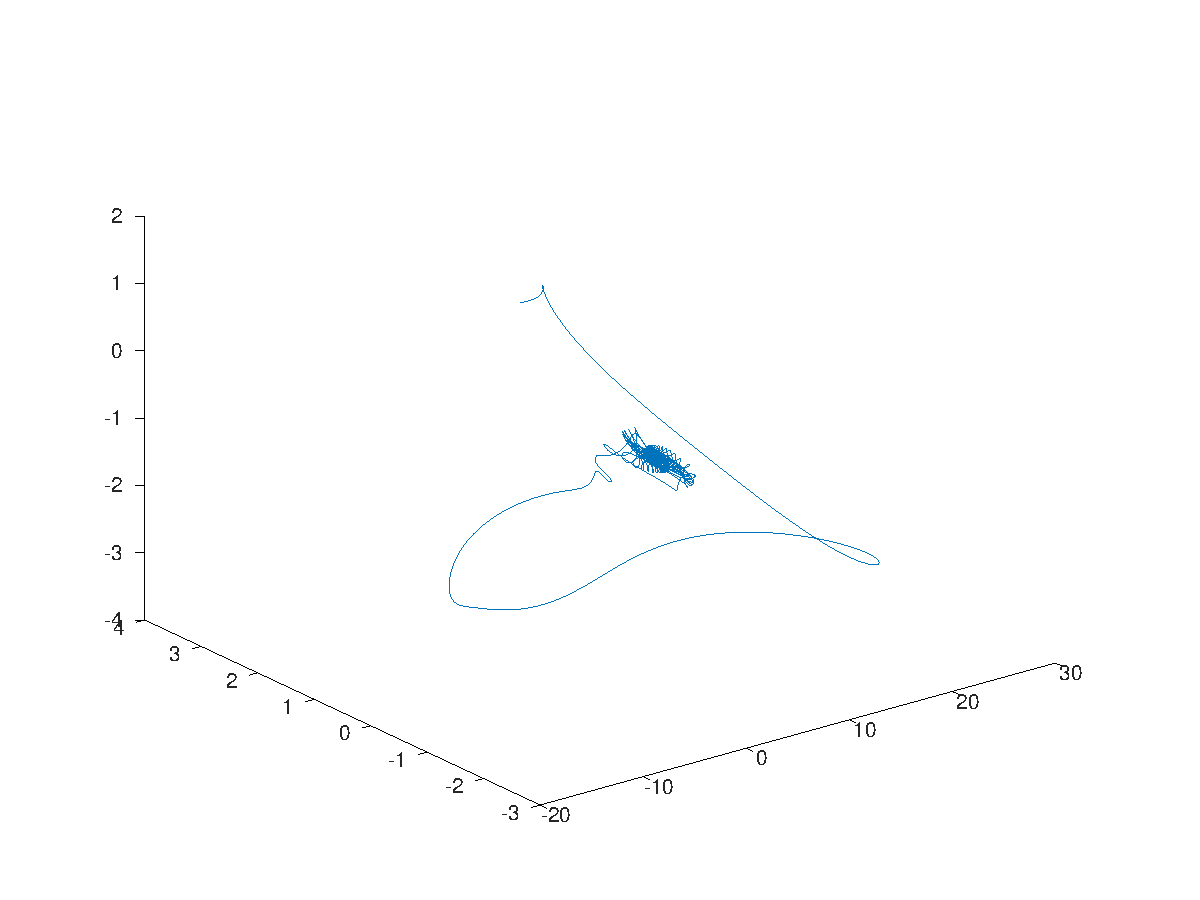
\includegraphics[width=0.49\linewidth]{{lorenz2/03-images/ord15.butterfly}.pdf}
	\caption{Lorenzssystem mit Grad 15, $t = [0,100]$}
	\label{figure:lorenz2:systemdeg15}
\end{figure}

\begin{figure}
	\centering
	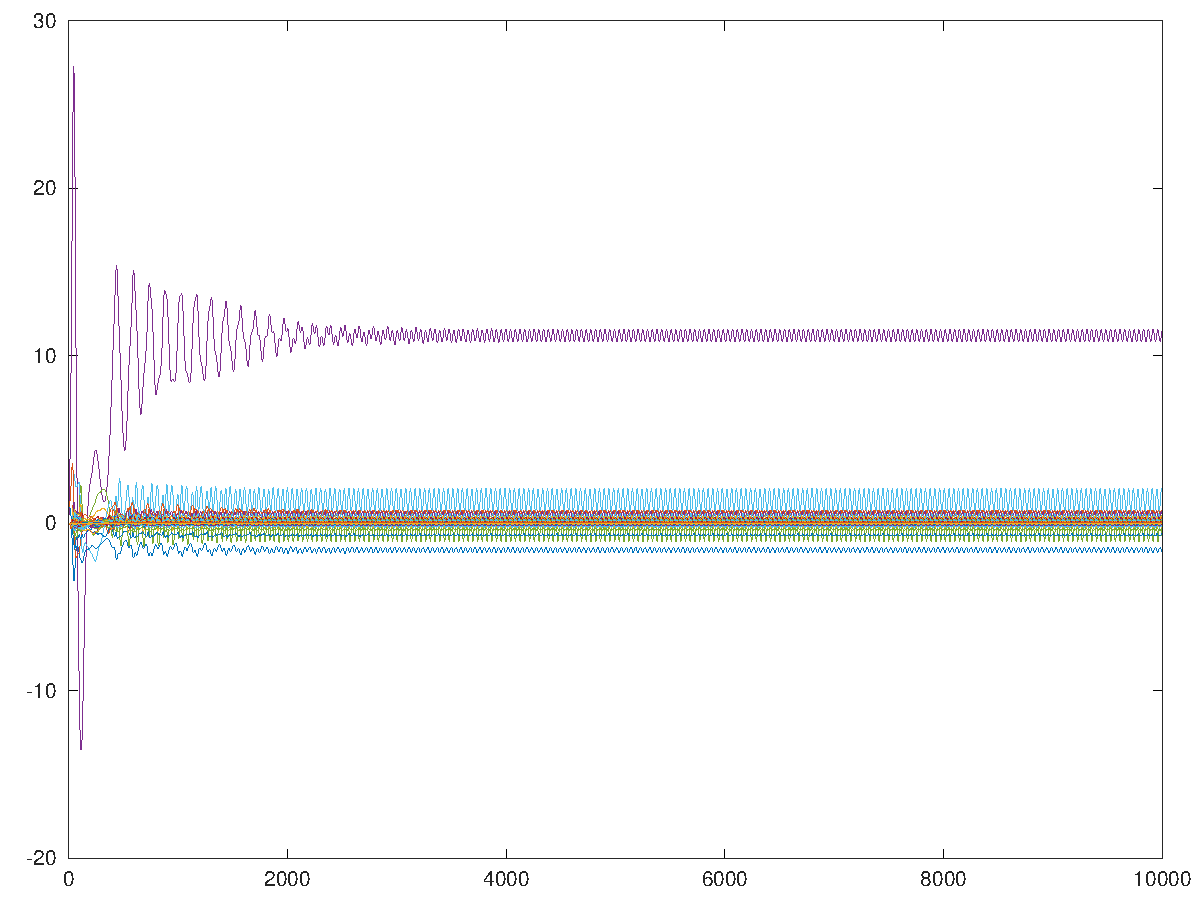
\includegraphics[width=0.49\linewidth]{{lorenz2/03-images/ord16.X}.pdf}
	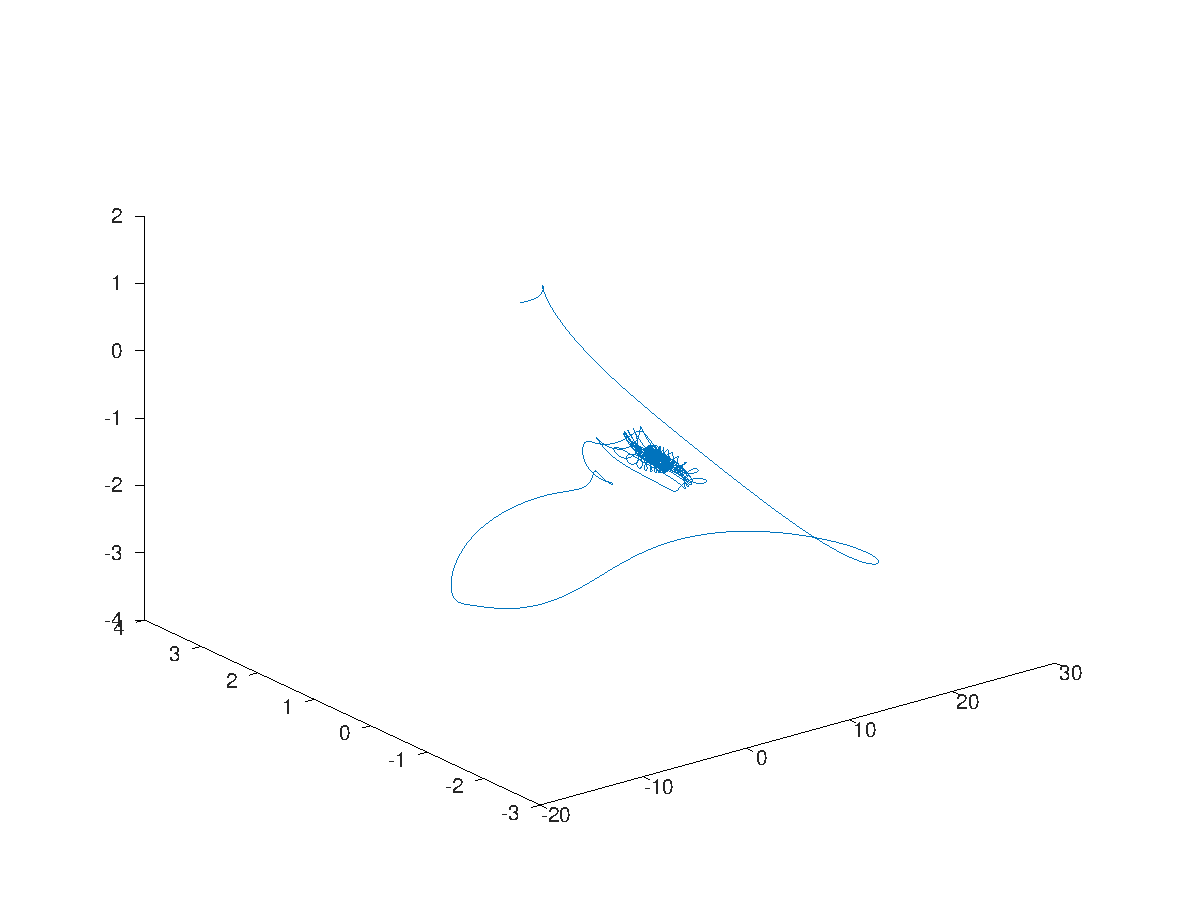
\includegraphics[width=0.49\linewidth]{{lorenz2/03-images/ord16.butterfly}.pdf}
	\caption{Lorenzssystem mit Grad 16, $t = [0,100]$}
	\label{figure:lorenz2:systemdeg16}
\end{figure}

\begin{figure}
	\centering
	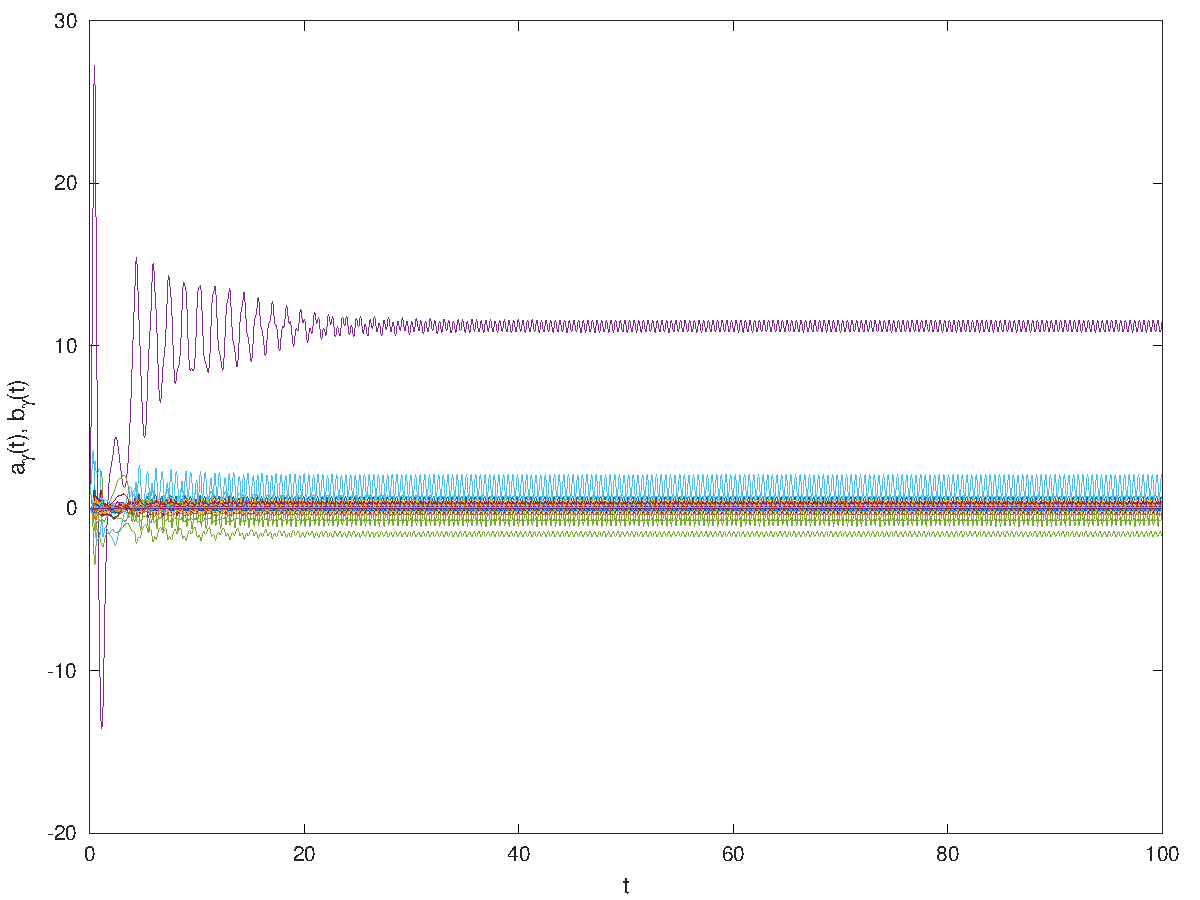
\includegraphics[width=0.49\linewidth]{{lorenz2/03-images/ord17.X}.pdf}
	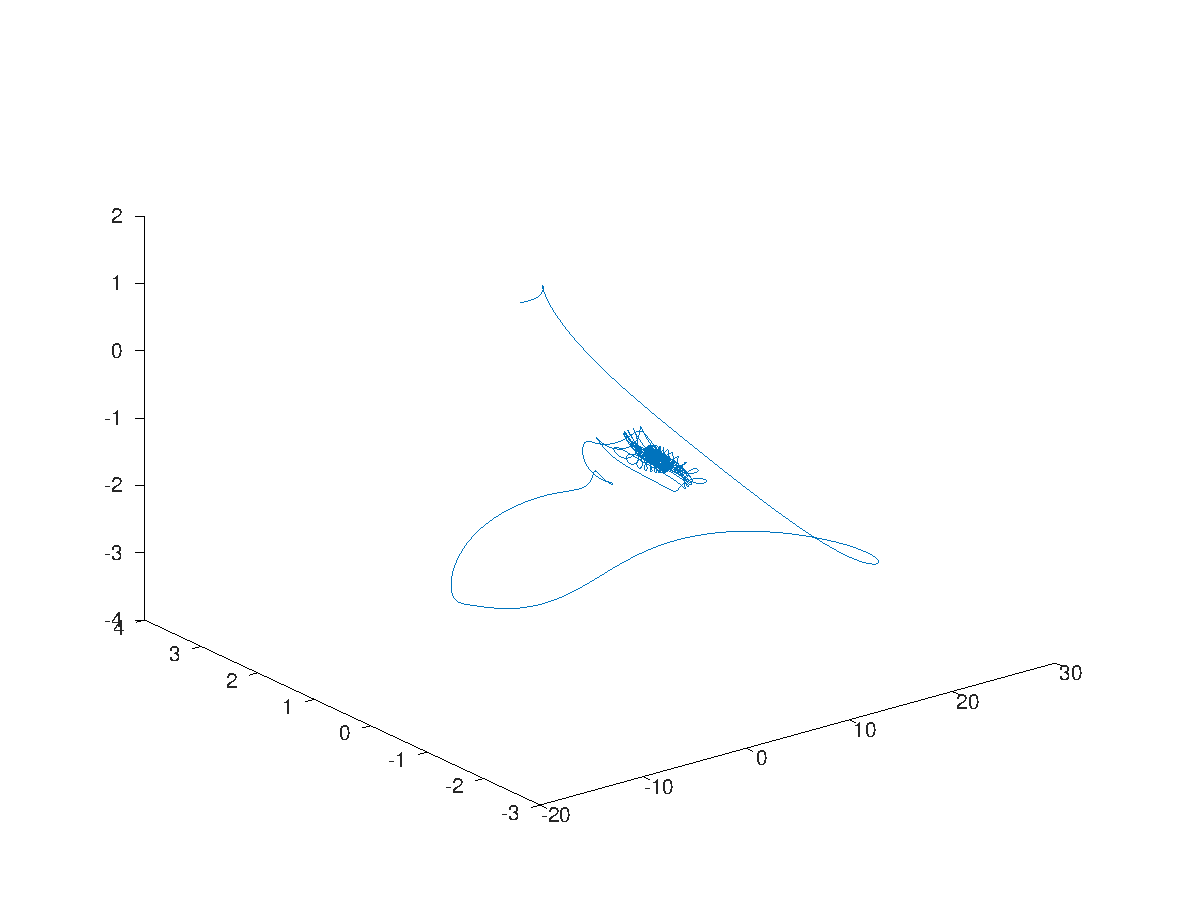
\includegraphics[width=0.49\linewidth]{{lorenz2/03-images/ord17.butterfly}.pdf}
	\caption{Lorenzssystem mit Grad 17, $t = [0,100]$}
	\label{figure:lorenz2:systemdeg17}
\end{figure}

\begin{figure}
	\centering
	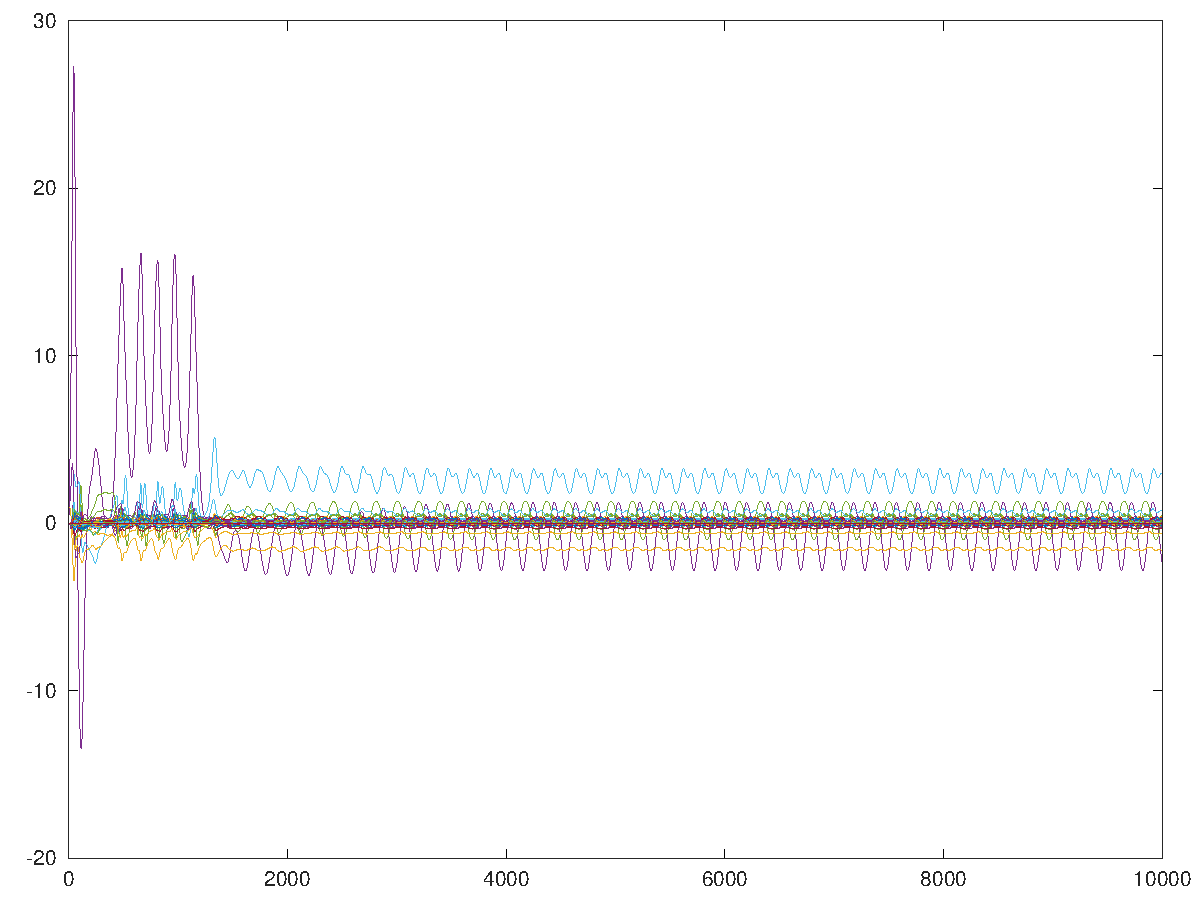
\includegraphics[width=0.49\linewidth]{{lorenz2/03-images/ord18.X}.pdf}
	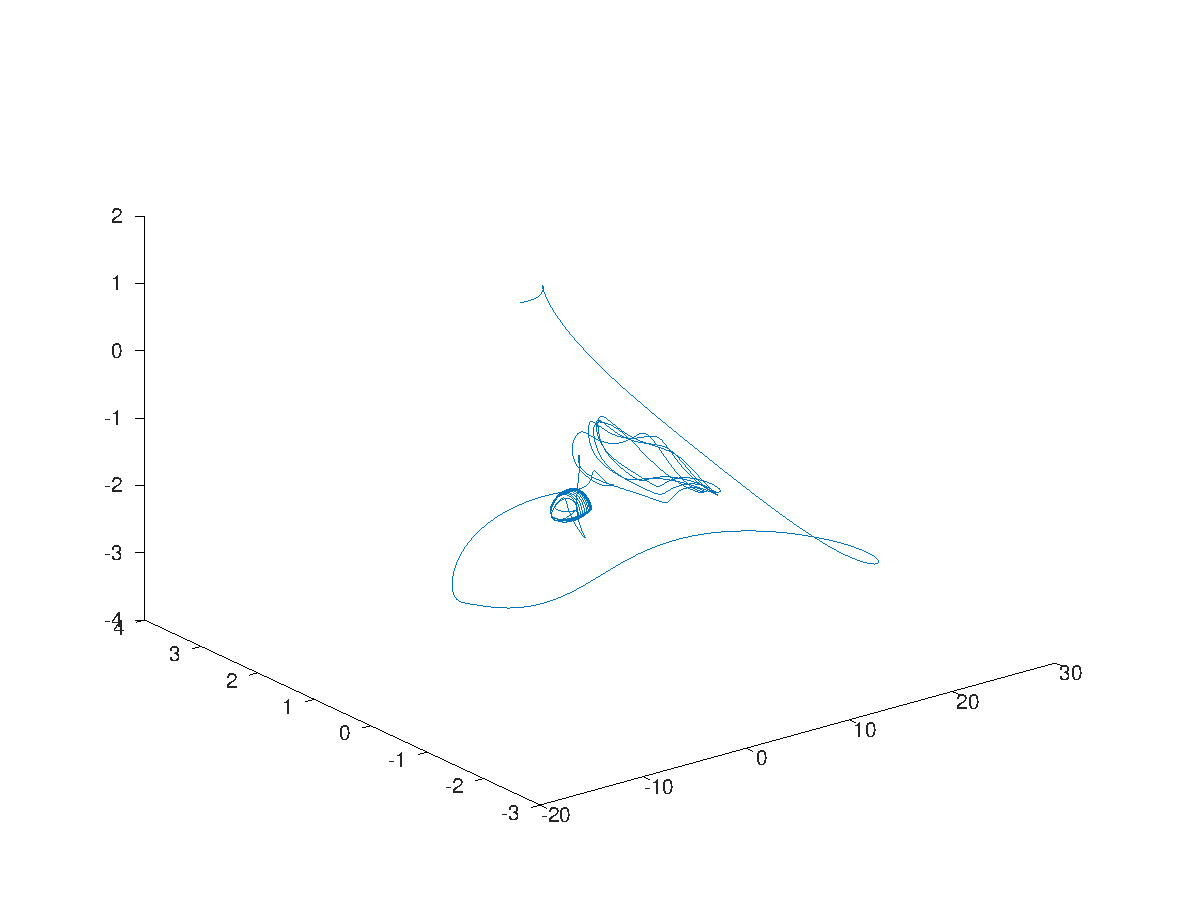
\includegraphics[width=0.49\linewidth]{{lorenz2/03-images/ord18.butterfly}.pdf}
	\caption{Lorenzssystem mit Grad 18, $t = [0,100]$}
	\label{figure:lorenz2:systemdeg18}
\end{figure}

\begin{figure}
	\centering
	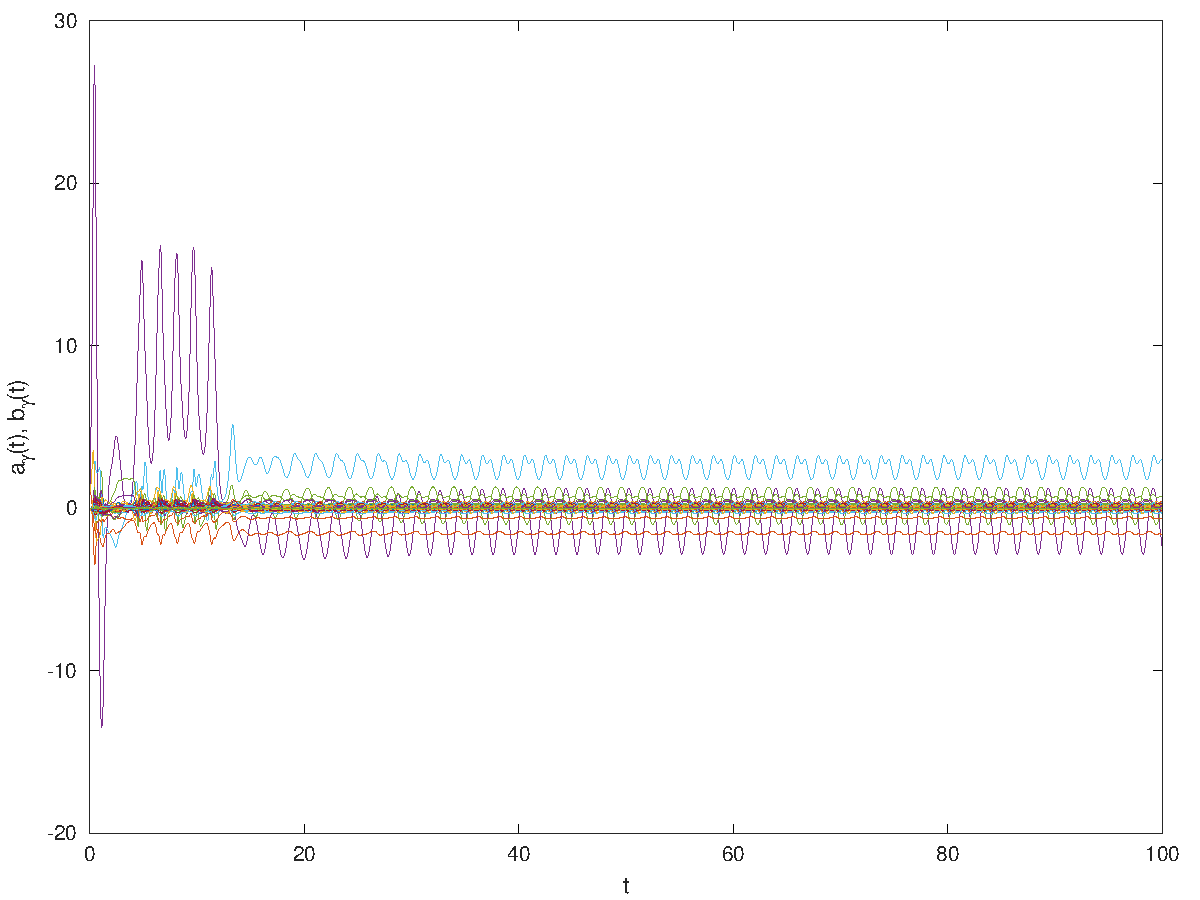
\includegraphics[width=0.49\linewidth]{{lorenz2/03-images/ord19.X}.pdf}
	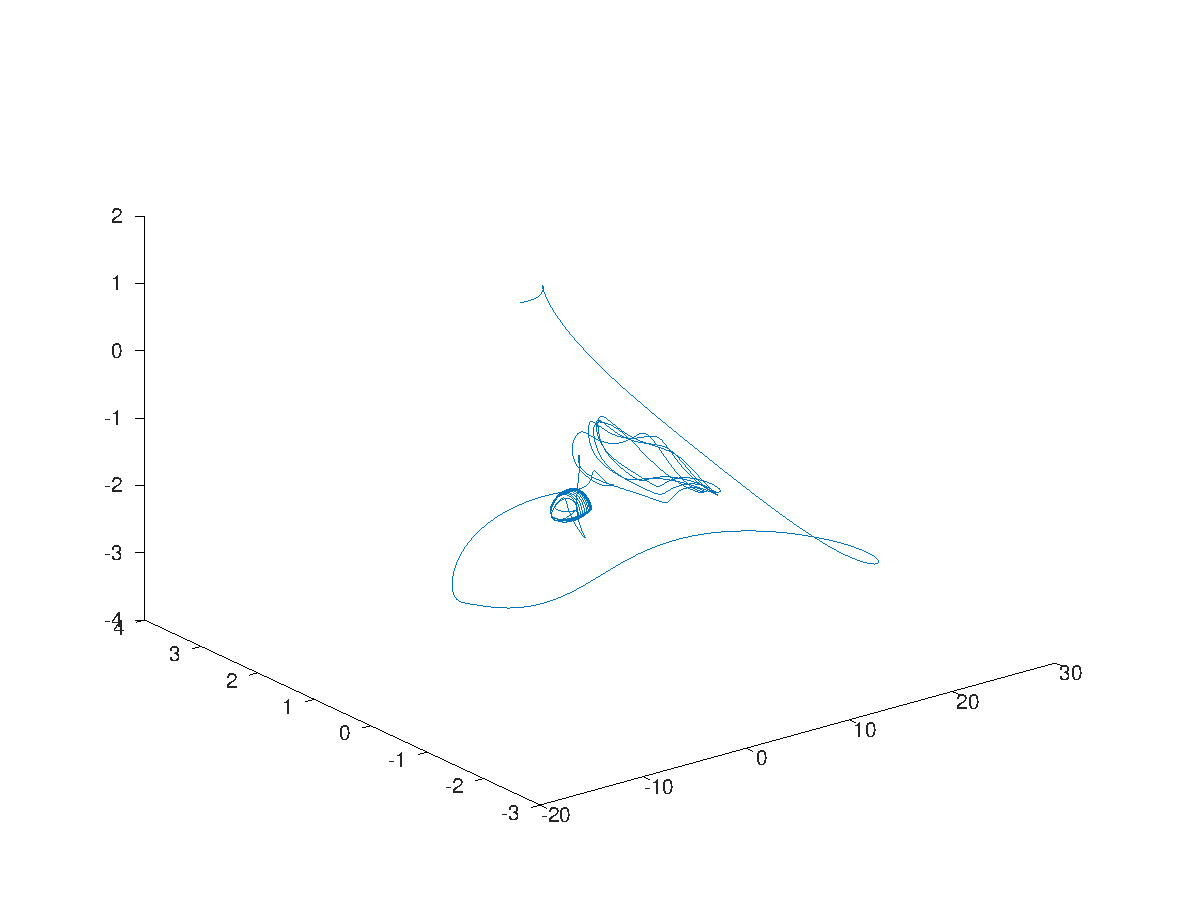
\includegraphics[width=0.49\linewidth]{{lorenz2/03-images/ord19.butterfly}.pdf}
	\caption{Lorenzssystem mit Grad 19, $t = [0,100]$}
	\label{figure:lorenz2:systemdeg19}
\end{figure}

\begin{figure}
	\centering
	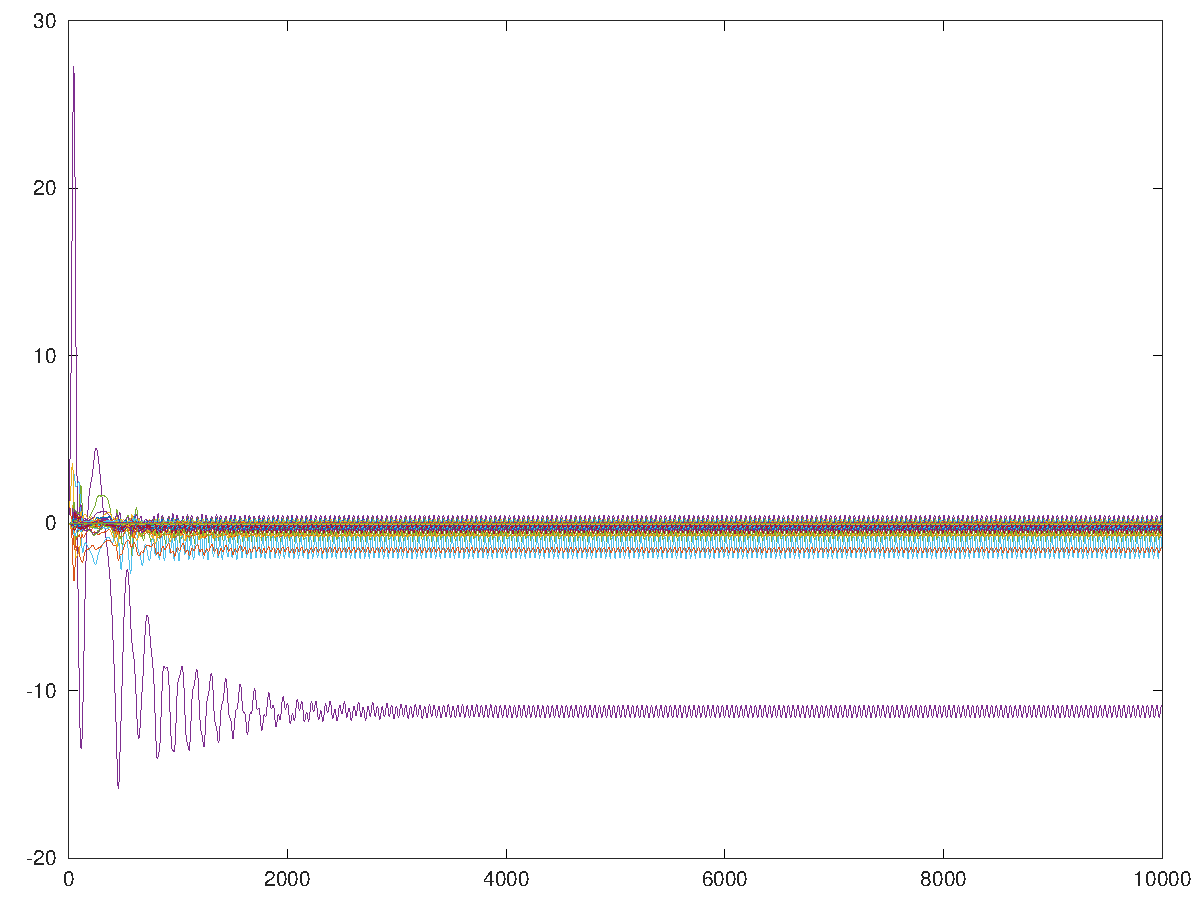
\includegraphics[width=0.49\linewidth]{{lorenz2/03-images/ord20.X}.pdf}
	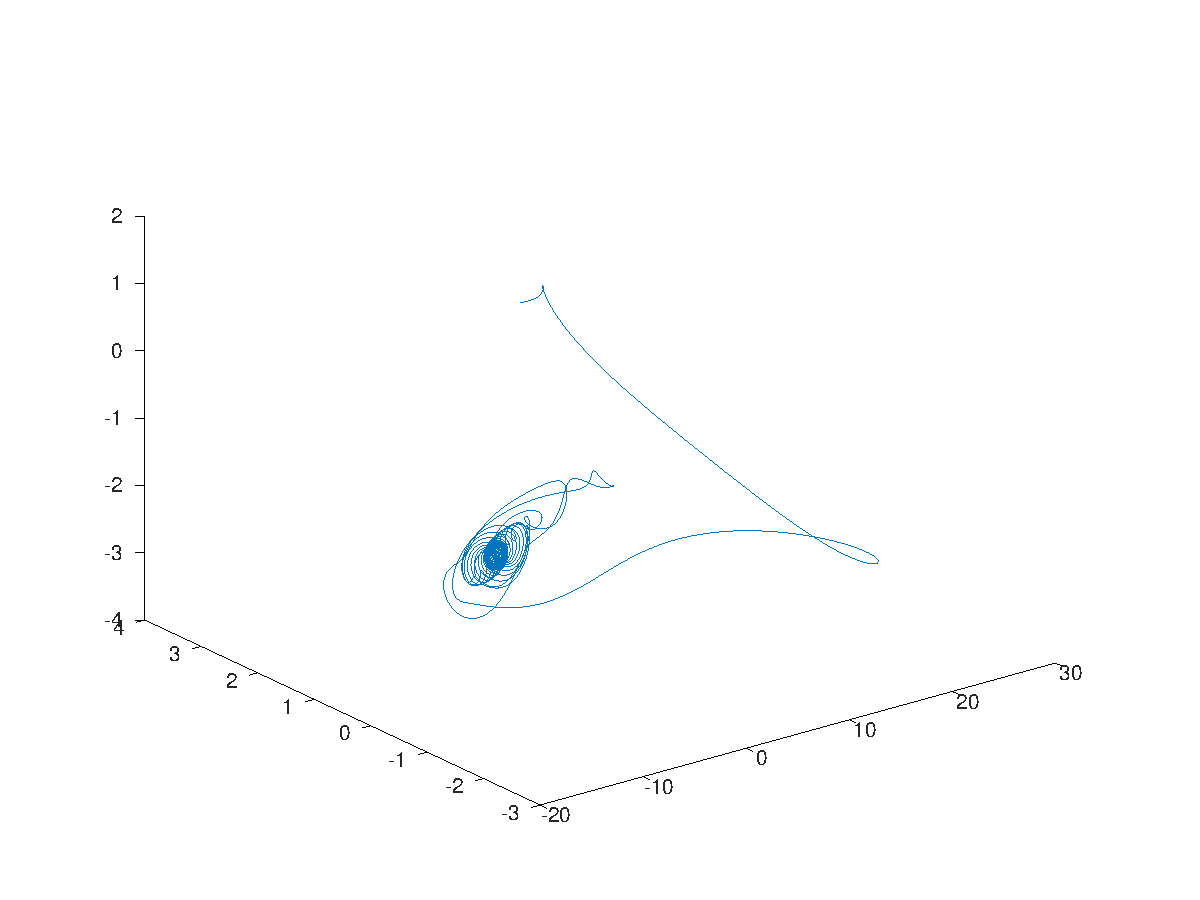
\includegraphics[width=0.49\linewidth]{{lorenz2/03-images/ord20.butterfly}.pdf}
	\caption{Lorenzssystem mit Grad 20, $t = [0,100]$}
	\label{figure:lorenz2:systemdeg20}
\end{figure}

\begin{figure}
	\centering
	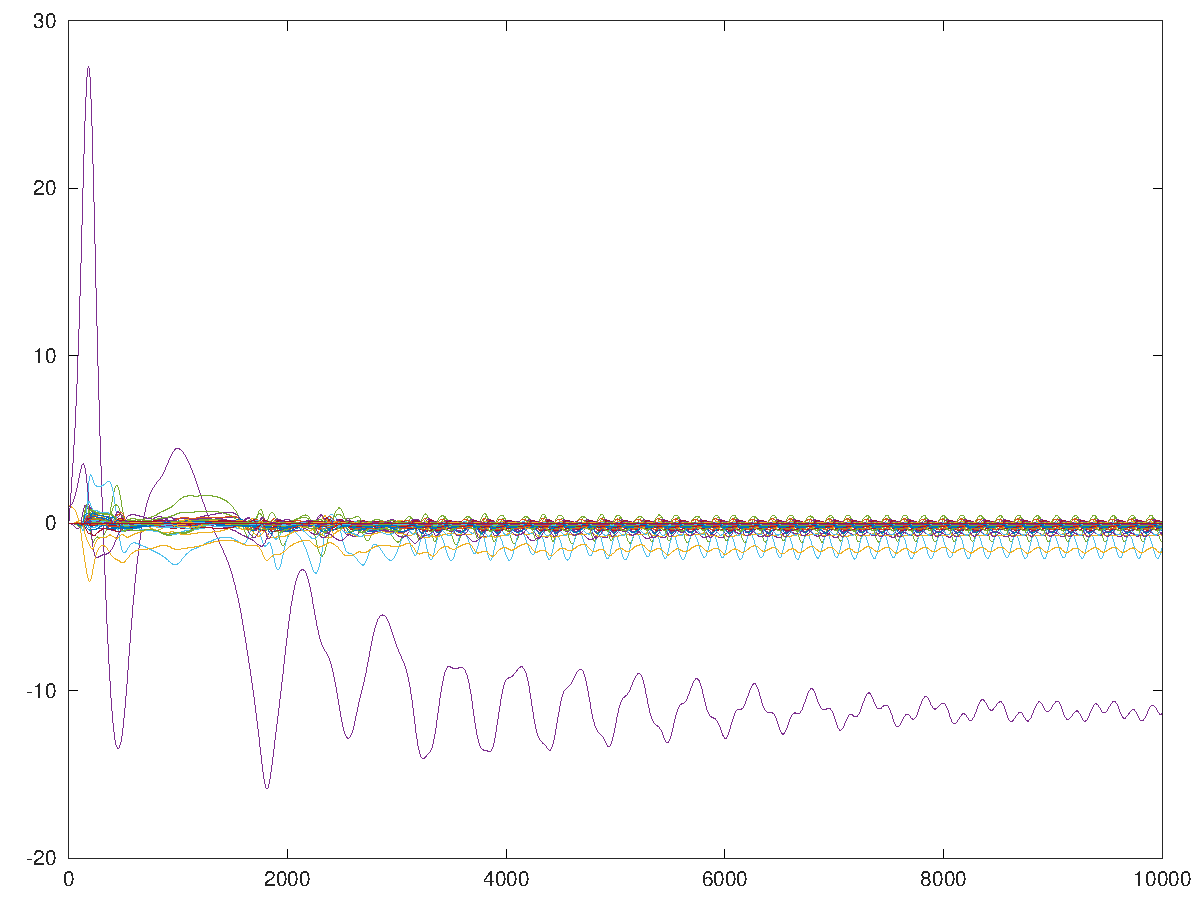
\includegraphics[width=0.49\linewidth]{{lorenz2/03-images/ord21.X.40}.pdf}
	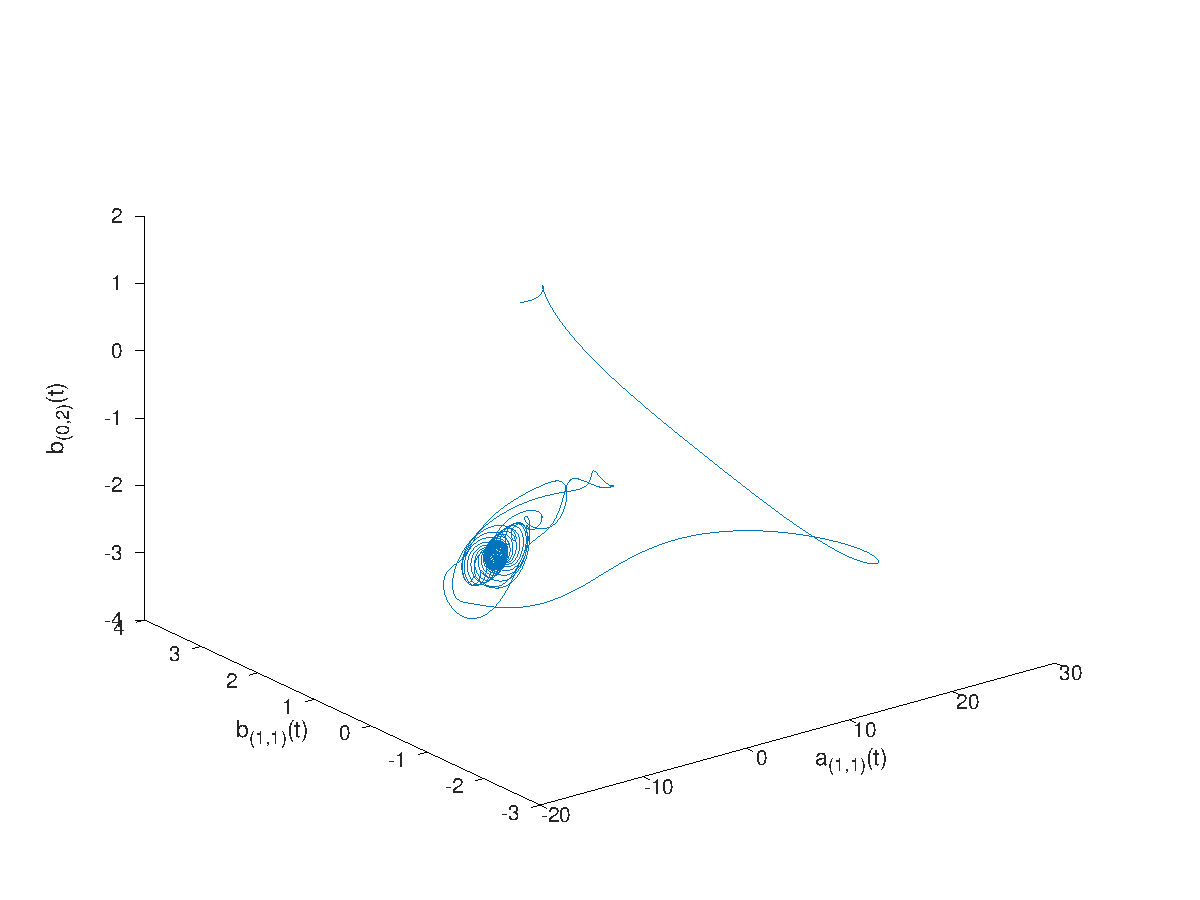
\includegraphics[width=0.49\linewidth]{{lorenz2/03-images/ord21.butterfly.40}.pdf}
	\caption{Lorenzssystem mit Grad 21, $t = [0,40]$}
	\label{figure:lorenz2:systemdeg21-40}
\end{figure}

\begin{figure}
	\centering
	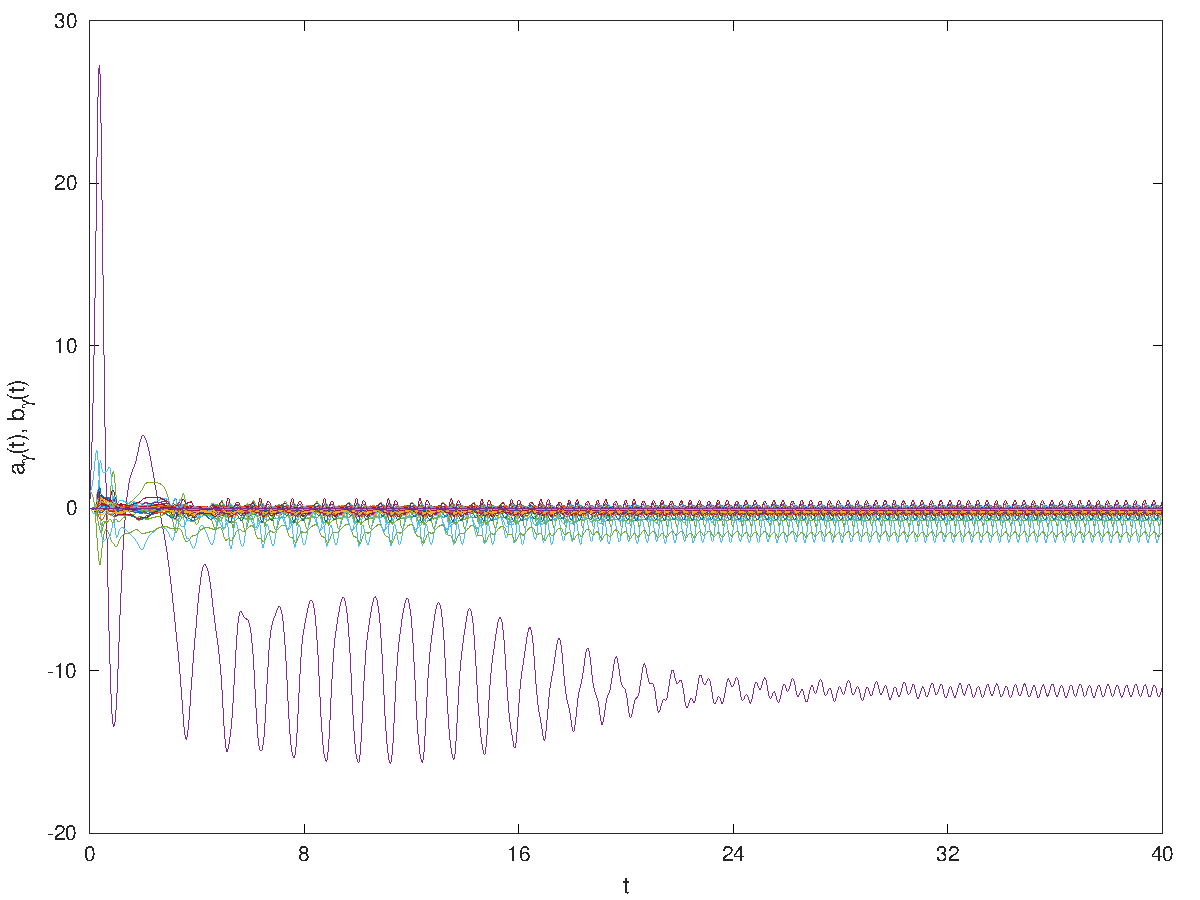
\includegraphics[width=0.49\linewidth]{{lorenz2/03-images/ord22.X.40}.pdf}
	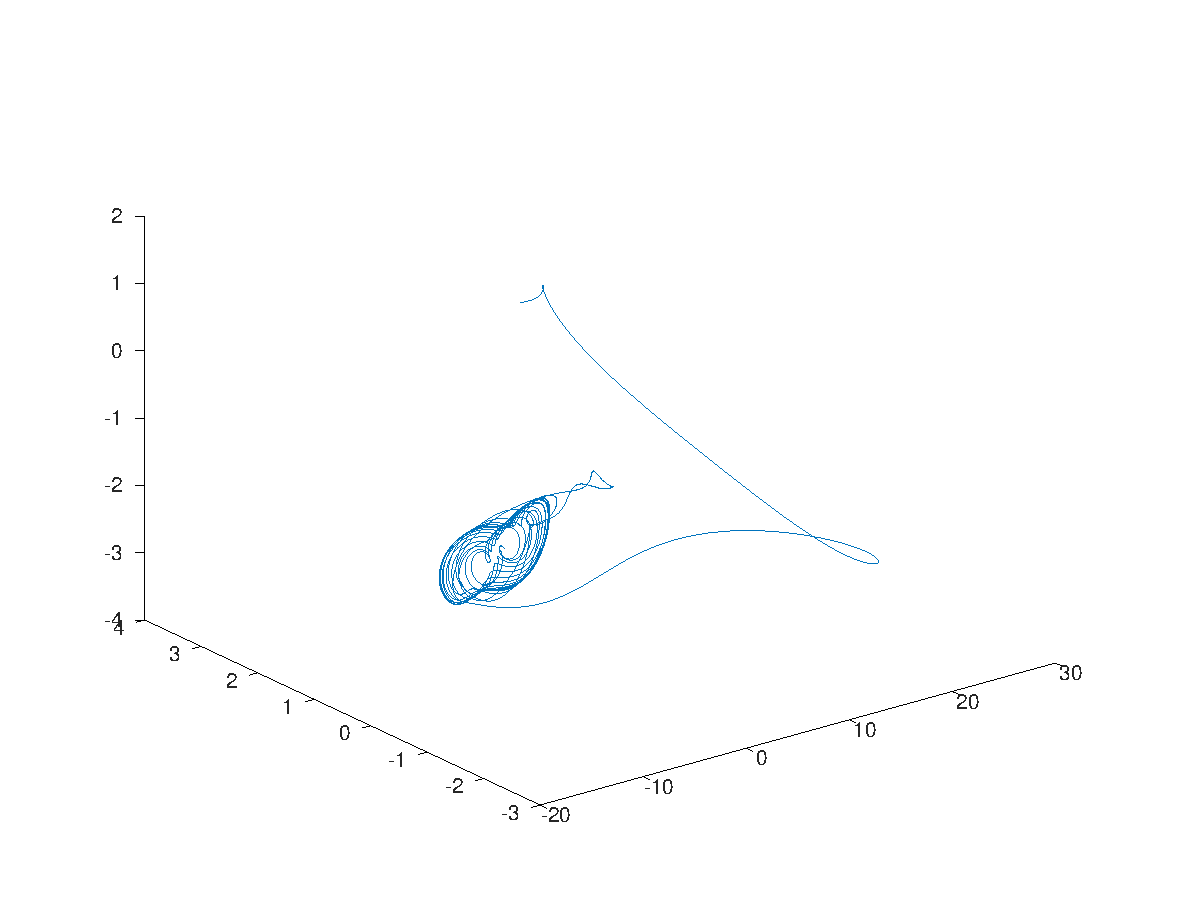
\includegraphics[width=0.49\linewidth]{{lorenz2/03-images/ord22.butterfly.40}.pdf}
	\caption{Lorenzssystem mit Grad 22, $t = [0,40]$}
	\label{figure:lorenz2:systemdeg22-40}
\end{figure}
